% version 1.2 dated 09 May 2011

% This file (c) 2009-2011 Elsevier Ltd.  Modifications may be freely made,
% provided the edited file is saved under a different name

% This file contains modifications for Procedia Computer Science

% Changes since version 1.1
% - added "procedia" option compliant with ecrc.sty version 1.2a
%   (makes the layout approximately the same as the Word CRC template)
% - added example for generating copyright line in abstract

%-----------------------------------------------------------------------------------

%% This template uses the elsarticle.cls document class and the extension package ecrc.sty
%% For full documentation on usage of elsarticle.cls, consult the documentation "elsdoc.pdf"
%% Further resources available at http://www.elsevier.com/latex

%-----------------------------------------------------------------------------------

%%%%%%%%%%%%%%%%%%%%%%%%%%%%%%%%%%%%%%%%%%%%%%%%%%%%%%%%%%%%%%
%%%%%%%%%%%%%%%%%%%%%%%%%%%%%%%%%%%%%%%%%%%%%%%%%%%%%%%%%%%%%%
%%                                                          %%
%% Important note on usage                                  %%
%% -----------------------                                  %%
%% This file should normally be compiled with PDFLaTeX      %%
%% Using standard LaTeX should work but may produce clashes %%
%%                                                          %%
%%%%%%%%%%%%%%%%%%%%%%%%%%%%%%%%%%%%%%%%%%%%%%%%%%%%%%%%%%%%%%
%%%%%%%%%%%%%%%%%%%%%%%%%%%%%%%%%%%%%%%%%%%%%%%%%%%%%%%%%%%%%%

%% The '3p' and 'times' class options of elsarticle are used for Elsevier CRC
%% The 'procedia' option causes ecrc to approximate to the Word template
\documentclass[3p,times,procedia]{elsarticle}
\flushbottom

%% The `ecrc' package must be called to make the CRC functionality available
\usepackage{ecrc}
%\usepackage{parskip}
\usepackage{amsmath}
\usepackage{ragged2e}
\usepackage{graphicx}
\usepackage{float}
\usepackage{listings}
\usepackage{color}
\usepackage{caption}
\usepackage{multicol}
\usepackage{titlesec}

% \titleformat*{\section}{\LARGE\bfseries}
\titleformat*{\subsection}{\Large\bfseries}
\titleformat*{\subsubsection}{\large\bfseries}

\captionsetup[figure]{font=normalsize}

% \lstset{basicstyle=\ttfamily, keywordstyle=\bfseries}
\definecolor{mygreen}{rgb}{0,0.6,0}
\definecolor{mygray}{rgb}{0.5,0.5,0.5}
\definecolor{mymauve}{rgb}{0.58,0,0.82}

\lstset{ %
  backgroundcolor=\color{white},   % choose the background color
  basicstyle=\scriptsize,        % size of fonts used for the code
  breaklines=true,                 % automatic line breaking only at whitespace
  captionpos=b,                    % sets the caption-position to bottom
  commentstyle=\color{mygreen},    % comment style
  escapeinside={\%*}{*)},          % if you want to add LaTeX within your code
  keywordstyle=\color{blue},       % keyword style
  stringstyle=\color{mymauve},     % string literal style
}



\definecolor{darkred}{rgb}{0.6,0.0,0.0}
\definecolor{darkgreen}{rgb}{0,0.50,0}
\definecolor{lightblue}{rgb}{0.0,0.42,0.91}
\definecolor{orange}{rgb}{0.99,0.48,0.13}
\definecolor{grass}{rgb}{0.18,0.80,0.18}
\definecolor{pink}{rgb}{0.97,0.15,0.45}

% listings
\usepackage{listings}

% General Setting of listings
\lstset{
  aboveskip=1em,
  breaklines=true,
  abovecaptionskip=-6pt,
  captionpos=b,
  escapeinside={\%*}{*)},
  frame=single,
%   numbers=left,
  numbersep=15pt,
  numberstyle=\tiny,
}
% 0. Basic Color Theme
% \lstdefinestyle{colored}{ %
%   basicstyle=\ttfamily,
%   backgroundcolor=\color{white},
%   commentstyle=\color{green}\itshape,
%   keywordstyle=\color{blue}\bfseries\itshape,
%   stringstyle=\color{red},
% }
% 1. General Python Keywords List
\lstdefinelanguage{PythonPlus}[]{Python}{
  morekeywords=[1]{,as,assert,nonlocal,with,yield,self,True,False,None,} % Python builtin
  morekeywords=[2]{,__init__,__add__,__mul__,__div__,__sub__,__call__,__getitem__,__setitem__,__eq__,__ne__,__nonzero__,__rmul__,__radd__,__repr__,__str__,__get__,__truediv__,__pow__,__name__,__future__,__all__,}, % magic methods
  morekeywords=[3]{,object,type,isinstance,copy,deepcopy,zip,enumerate,reversed,list,set,len,dict,tuple,range,xrange,append,execfile,real,imag,reduce,str,repr,}, % common functions
  morekeywords=[4]{,Exception,NameError,IndexError,SyntaxError,TypeError,ValueError,OverflowError,ZeroDivisionError,}, % errors
  morekeywords=[5]{,ode,fsolve,sqrt,exp,sin,cos,arctan,arctan2,arccos,pi, array,norm,solve,dot,arange,isscalar,max,sum,flatten,shape,reshape,find,any,all,abs,plot,linspace,legend,quad,polyval,polyfit,hstack,concatenate,vstack,column_stack,empty,zeros,ones,rand,vander,grid,pcolor,eig,eigs,eigvals,svd,qr,tan,det,logspace,roll,min,mean,cumsum,cumprod,diff,vectorize,lstsq,cla,eye,xlabel,ylabel,squeeze,}, % numpy / math
}
% 2. New Language based on Python
\lstdefinelanguage{PyBrIM}[]{PythonPlus}{
  emph={d,E,a,Fc28,Fy,Fu,D,des,supplier,Material,Rectangle,PyElmt},
}
% 3. Extended theme
\lstdefinestyle{colorEX}{
  basicstyle=\ttfamily,
  backgroundcolor=\color{white},
  commentstyle=\color{darkgreen}\slshape,
  keywordstyle=\color{blue}\bfseries\itshape,
  keywordstyle=[2]\color{blue}\bfseries,
  keywordstyle=[3]\color{grass},
  keywordstyle=[4]\color{red},
  keywordstyle=[5]\color{orange},
  stringstyle=\color{darkred},
  emphstyle=\color{pink}\underbar,
}



\newcommand{\subf}[2]{%
  {\small\begin{tabular}[t]{@{}c@{}}
  #1\\#2
  \end{tabular}}%
}

%% The ecrc package defines commands needed for running heads and logos.
%% For running heads, you can set the journal name, the volume, the starting page and the authors

%% set the volume if you know. Otherwise `00'
%%\volume{}

%% set the starting page if not 1
\firstpage{1}

%% Give the name of the journal
\journalname{Computational Intelligence, Spring 2022}

%% Give the author list to appear in the running head
%% Example \runauth{C.V. Radhakrishnan et al.}
\runauth{}

%% The choice of journal logo is determined by the \jid and \jnltitlelogo commands.
%% A user-supplied logo with the name <\jid>logo.pdf will be inserted if present.
%% e.g. if \jid{yspmi} the system will look for a file yspmilogo.pdf
%% Otherwise the content of \jnltitlelogo will be set between horizontal lines as a default logo

%% Give the abbreviation of the Journal.
%% \jid{}

%% Give a short journal name for the dummy logo (if needed)
%\jnltitlelogo{Computer Science}

%% Hereafter the template follows `elsarticle'.
%% For more details see the existing template files elsarticle-template-harv.tex and elsarticle-template-num.tex.

%% Elsevier CRC generally uses a numbered reference style
%% For this, the conventions of elsarticle-template-num.tex should be followed (included below)
%% If using BibTeX, use the style file elsarticle-num.bst

%% End of ecrc-specific commands
%%%%%%%%%%%%%%%%%%%%%%%%%%%%%%%%%%%%%%%%%%%%%%%%%%%%%%%%%%%%%%%%%%%%%%%%%%

%% The amssymb package provides various useful mathematical symbols

\usepackage{amssymb}
%% The amsthm package provides extended theorem environments
%% \usepackage{amsthm}

%% The lineno packages adds line numbers. Start line numbering with
%% \begin{linenumbers}, end it with \end{linenumbers}. Or switch it on
%% for the whole article with \linenumbers after \end{frontmatter}.
%% \usepackage{lineno}

%% natbib.sty is loaded by default. However, natbib options can be
%% provided with \biboptions{...} command. Following options are
%% valid:

%%   round  -  round parentheses are used (default)
%%   square -  square brackets are used   [option]
%%   curly  -  curly braces are used      {option}
%%   angle  -  angle brackets are used    <option>
%%   semicolon  -  multiple citations separated by semi-colon
%%   colon  - same as semicolon, an earlier confusion
%%   comma  -  separated by comma
%%   numbers-  selects numerical citations
%%   super  -  numerical citations as superscripts
%%   sort   -  sorts multiple citations according to order in ref. list
%%   sort&compress   -  like sort, but also compresses numerical citations
%%   compress - compresses without sorting
%%
%% \biboptions{authoryear}

% \biboptions{}

% if you have landscape tables
\usepackage[figuresright]{rotating}
%\usepackage{harvard}
% put your own definitions here:x
%   \newcommand{\cZ}{\cal{Z}}
%   \newtheorem{def}{Definition}[section]
%   ...

% add words to TeX's hyphenation exception list
%\hyphenation{author another created financial paper re-commend-ed Post-Script}

% declarations for front matter


\begin{document}
\begin{frontmatter}

%% Title, authors and addresses

%% use the tnoteref command within \title for footnotes;
%% use the tnotetext command for the associated footnote;
%% use the fnref command within \author or \address for footnotes;
%% use the fntext command for the associated footnote;
%% use the corref command within \author for corresponding author footnotes;
%% use the cortext command for the associated footnote;
%% use the ead command for the email address,
%% and the form \ead[url] for the home page:
%%
%% \title{Title\tnoteref{label1}}
%% \tnotetext[label1]{}
%% \author{Name\corref{cor1}\fnref{label2}}
%% \ead{email address}
%% \ead[url]{home page}
%% \fntext[label2]{}
%% \cortext[cor1]{}
%% \address{Address\fnref{label3}}
%% \fntext[label3]{}

%\dochead{Middle East Technical University, Spring 2023}%

%% Use \dochead if there is an article header, e.g. \dochead{Short communication}
%% \dochead can also be used to include a conference title, if directed by the editors
%% e.g. \dochead{17th International Conference on Dynamical Processes in Excited States of Solids}

\title{\textbf{Evolutionary Art}}

%% use optional labels to link authors explicitly to addresses:
%% \author[label1,label2]{<author name>}
%% \address[label1]{<address>}
%% \address[label2]{<address>}



\author[]{Ozgur Gulsuna} 
%\author[b]{Second Author}
%\author[a,b]{Third Author\corref{cor1}}

\address[]{Middle East Technical University, Electrical and Electronics Engineering, Ankara, Turkey}
%\address[b]{Second affiliation, Address, City and Postcode, Country}

\begin{abstract}
%% Text of abstract

This report explores evolutionary algorithms for image generation problem given source image using filled circles. Individuals represent the population, with each gene corresponding to circle properties. Evaluation compares images using a fitness function. The process involves selection, crossover, and mutation. Experiments vary hyperparameters, analyzing fitness plots. Two modifications are proposed for improved convergence speed and quality.

\end{abstract}

\begin{keyword}
NumPy;
Evolutionary Algorithms;
Image Generation;
Vectorization

\end{keyword}

\end{frontmatter}

%\correspondingauthor[*]{Corresponding author. Tel.: +0-000-000-0000 ; fax: +0-000-000-0000.}
\email{ozgur.gulsuna@metu.edu.tr}

%%
%% Start line numbering here if you want
%%
% \linenumbers

%% main text

\enlargethispage{10mm}
\section{\textbf{Experiments with Hyperparameters}}
\label{main}

The first part of the report is about the hyperparameters. These are the parameters that are set by the designer and the values effect the output quality.
The hyperparameters are namely, population size, number of generations, mutation rate, crossover rate, and the number of circles.
Here an experiment is conducted to see the effect of these parameters on the output quality.
The default parameters are set as follows:
\begin{multicols}{3}
    \begin{itemize}
    \item Pop. Size: \textbf{20}
    \item Number of Genes: \textbf{50}  
    \item Tournament Size: \textbf{5}  
    \item Fraction of Elites: \textbf{0.2}
    \item Fraction of Parents: \textbf{0.6}
    \item Mutation Prob.: \textbf{0.2}
    \item Mutation Type: \textbf{guided}
    \item Generation Size: \textbf{10000}
    \end{itemize}
\end{multicols}
\begin{figure}[H]
    \centering
    \begin{tabular}{c c c c c c}
          \subf{
\includegraphics[width=20mm]{figures/def/cafe_terrace_at_night_gen_0.png}}{gens 0}
        &
        \subf{
\includegraphics[width=20mm]{figures/def/cafe_terrace_at_night_gen_999.png}}{gens 1000}
        &
        \subf{
\includegraphics[width=20mm]{figures/def/cafe_terrace_at_night_gen_1999.png}}{gens 2000}
        &
        \subf{
\includegraphics[width=20mm]{figures/def/cafe_terrace_at_night_gen_2999.png}}{gens 3000}
        &
        \subf{
\includegraphics[width=20mm]{figures/def/cafe_terrace_at_night_gen_3999.png}}{gens 4000}
        &
        \subf{
\includegraphics[width=20mm]{figures/def/cafe_terrace_at_night_gen_4999.png}}{gens 5000}
        \\
        \end{tabular}
    \begin{tabular}{c c c c c c}
        \subf{
\includegraphics[width=20mm]{figures/def/cafe_terrace_at_night_gen_5999.png}}{gens 6000}
        &
        \subf{
\includegraphics[width=20mm]{figures/def/cafe_terrace_at_night_gen_6999.png}}{gens 7000}
        &
        \subf{
\includegraphics[width=20mm]{figures/def/cafe_terrace_at_night_gen_7999.png}}{gens 8000}
        &
        \subf{
\includegraphics[width=20mm]{figures/def/cafe_terrace_at_night_gen_8999.png}}{gens 9000}
        &
        \subf{
\includegraphics[width=20mm]{figures/def/cafe_terrace_at_night_gen_9999.png}}{gens 10000}
        &
        \subf{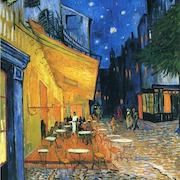
\includegraphics[width=20mm]{figures/cafe_terrace_at_night.png}}{original}
        \\
        \end{tabular}
\caption{ Best Images for Default Parameters}
\normalsize
\end{figure}

\begin{figure}[H]
    \centering
    \begin{tabular}{c c}
        \subf{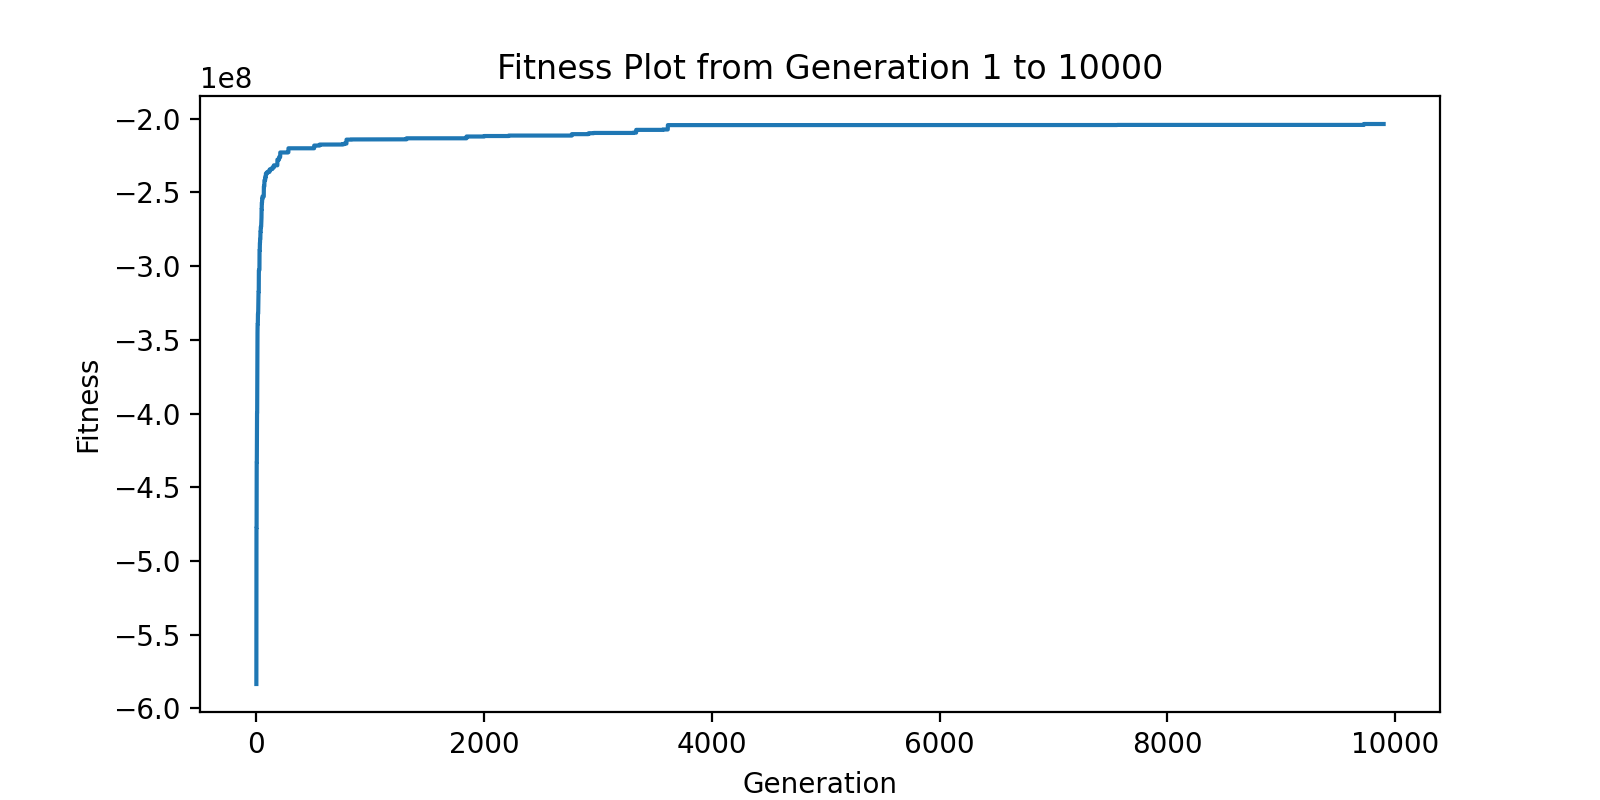
\includegraphics[width=75mm]{figures/def/cafe_terrace_at_night_fitness.png}}{gens 1 to 10000}
        &
        \subf{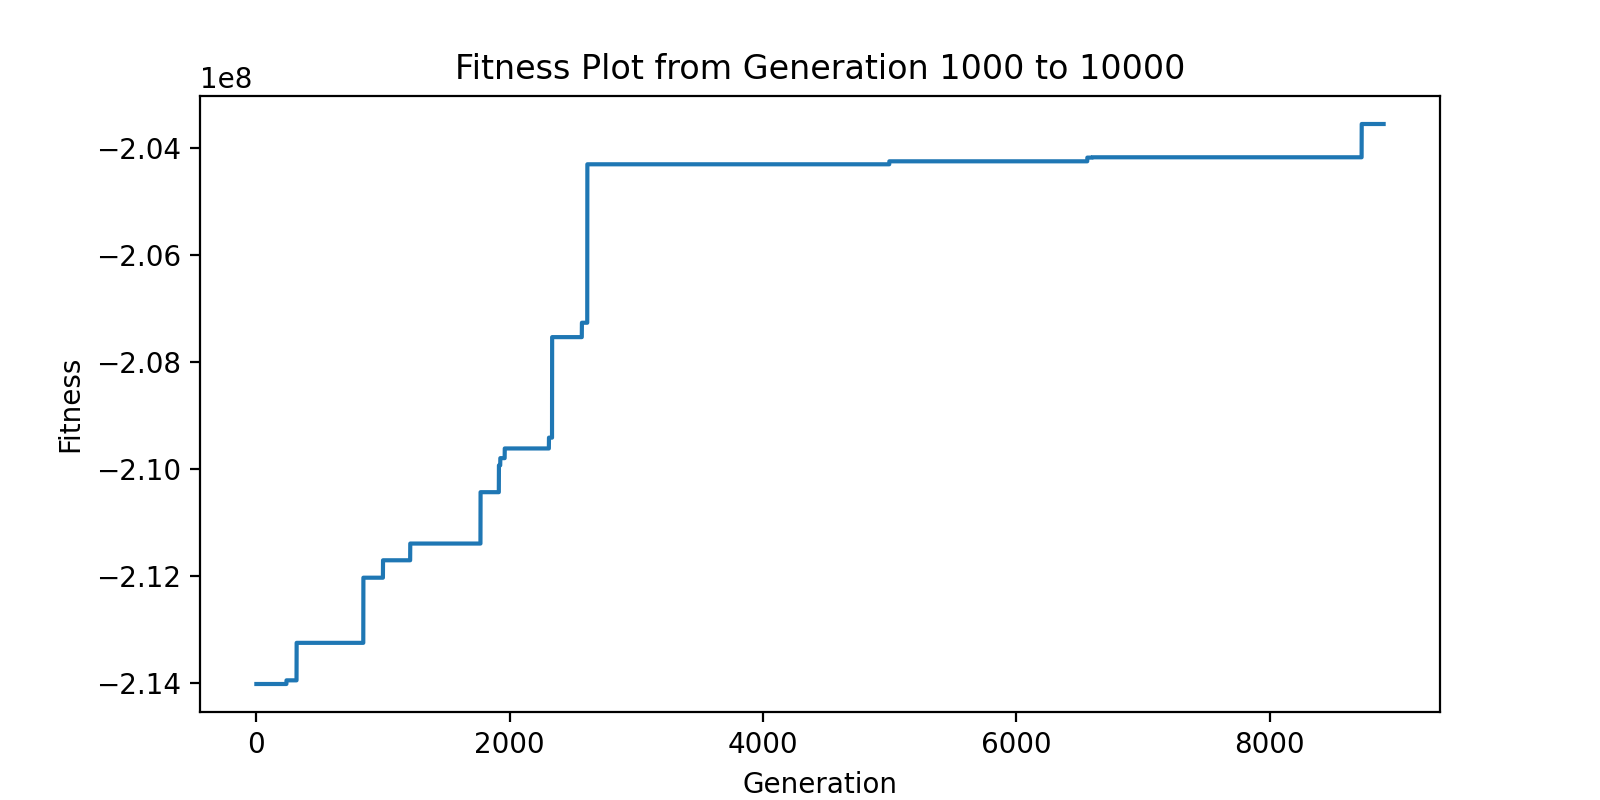
\includegraphics[width=75mm]{figures/def/cafe_terrace_at_night_fitness_1000.png}}{gens 1000 to 10000}
        \\
        \end{tabular}
\caption{ Fitness Plots for Default Parameters}
\normalsize
\end{figure}



\subsection{\textbf{\Large Number of Individuals \(<num\_inds>\)}}

The number of individuals is the size of the population. The individuals are used to generate next generation.
Higher the number of individuals, the more diverse the starting population is.

\subsubsection{\textbf{Number of Individuals  = 5}}

\begin{figure}[H]
    \centering
    \begin{tabular}{c c c c c c}
          \subf{
\includegraphics[width=20mm]{figures/ind-5/cafe_terrace_at_night_gen_0.png}}{gens 0}
        &
        \subf{
\includegraphics[width=20mm]{figures/ind-5/cafe_terrace_at_night_gen_999.png}}{gens 1000}
        &
        \subf{
\includegraphics[width=20mm]{figures/ind-5/cafe_terrace_at_night_gen_1999.png}}{gens 2000}
        &
        \subf{
\includegraphics[width=20mm]{figures/ind-5/cafe_terrace_at_night_gen_2999.png}}{gens 3000}
        &
        \subf{
\includegraphics[width=20mm]{figures/ind-5/cafe_terrace_at_night_gen_3999.png}}{gens 4000}
        &
        \subf{
\includegraphics[width=20mm]{figures/ind-5/cafe_terrace_at_night_gen_4999.png}}{gens 5000}
        \\
        \end{tabular}
    \begin{tabular}{c c c c c c}
        \subf{
\includegraphics[width=20mm]{figures/ind-5/cafe_terrace_at_night_gen_5999.png}}{gens 6000}
        &
        \subf{
\includegraphics[width=20mm]{figures/ind-5/cafe_terrace_at_night_gen_6999.png}}{gens 7000}
        &
        \subf{
\includegraphics[width=20mm]{figures/ind-5/cafe_terrace_at_night_gen_7999.png}}{gens 8000}
        &
        \subf{
\includegraphics[width=20mm]{figures/ind-5/cafe_terrace_at_night_gen_8999.png}}{gens 9000}
        &
        \subf{
\includegraphics[width=20mm]{figures/ind-5/cafe_terrace_at_night_gen_9999.png}}{gens 10000}
        &
        \subf{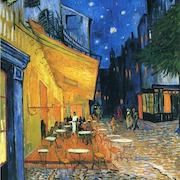
\includegraphics[width=20mm]{figures/cafe_terrace_at_night.png}}{original}
        \\
        \end{tabular}
\caption{ Best Images for $<num\_inds>$ = 5}
\normalsize
\end{figure}

\begin{figure}[H]
    \centering
    \begin{tabular}{c c}
        \subf{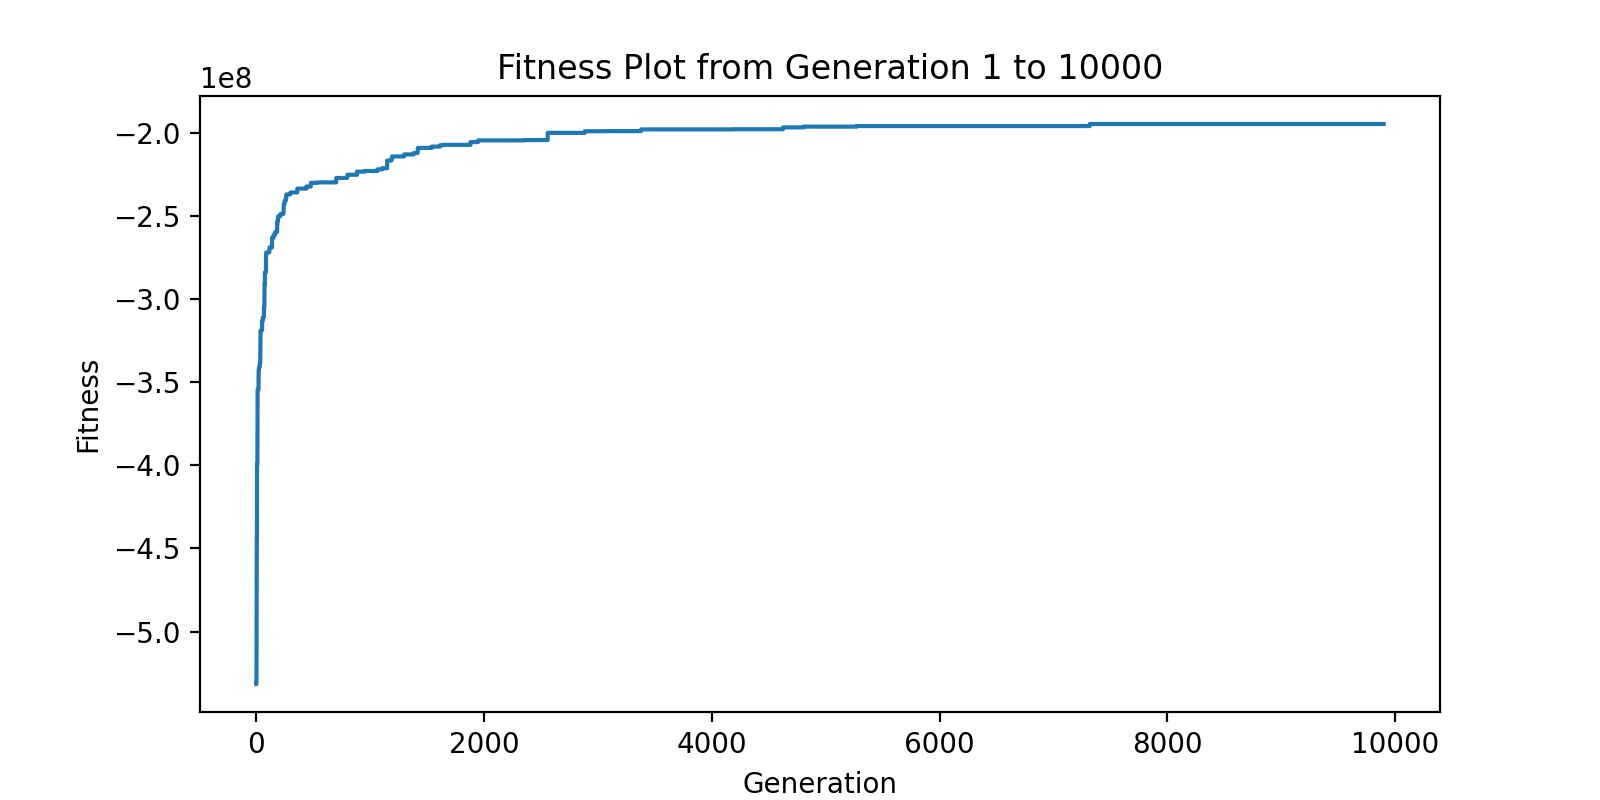
\includegraphics[width=75mm]{figures/ind-5/cafe_terrace_at_night_fitness.png}}{gens 1 to 10000}
        &
        \subf{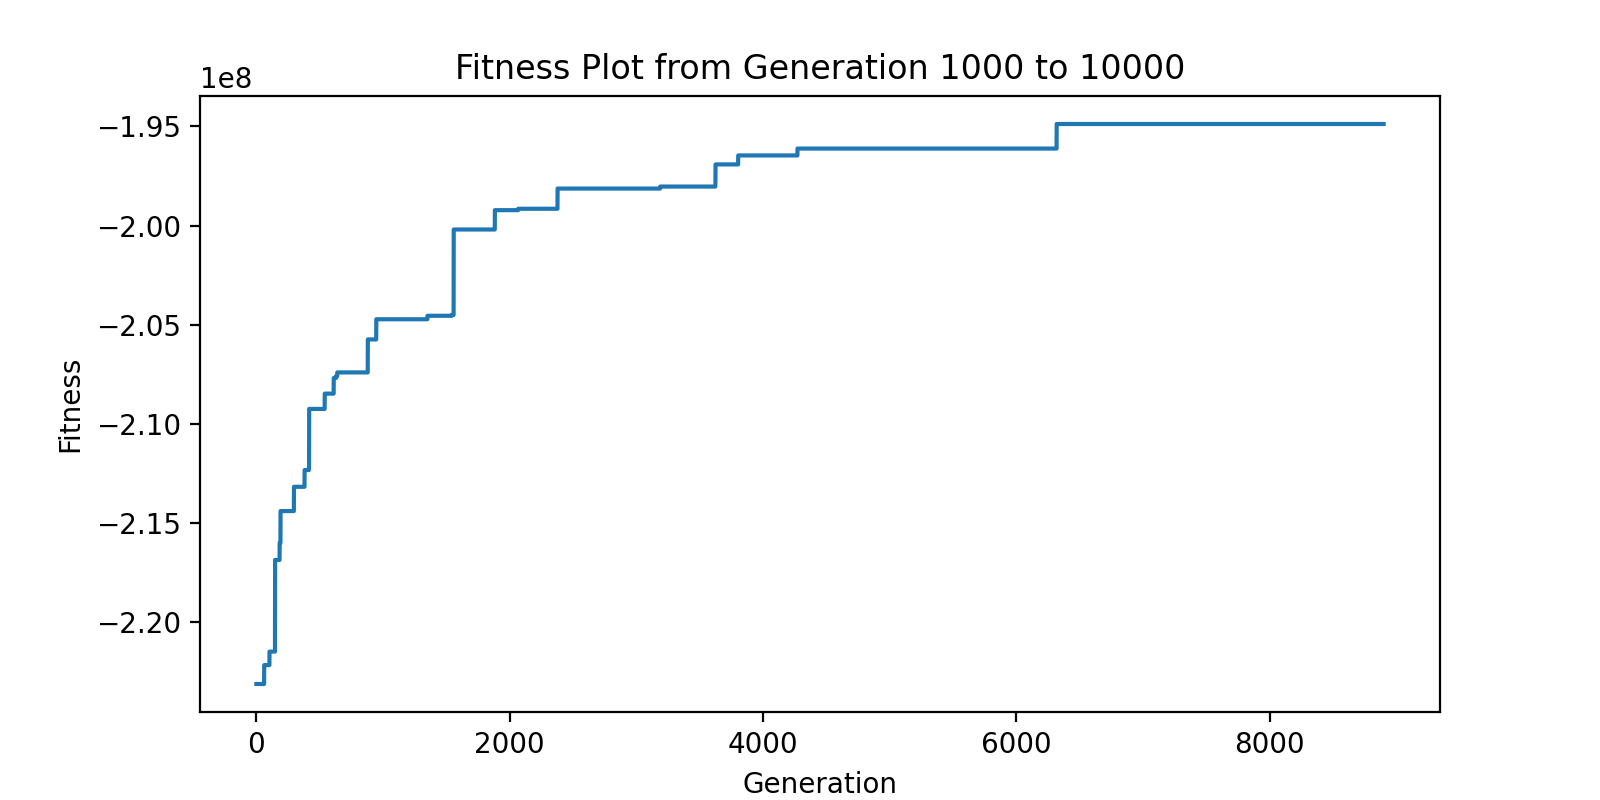
\includegraphics[width=75mm]{figures/ind-5/cafe_terrace_at_night_fitness_1000.png}}{gens 1000 to 10000}
        \\
        \end{tabular}
\caption{ Fitness Plots for $<num\_inds>$ = 5}
\normalsize
\end{figure}

\subsubsection{\textbf{Number of Individuals  = 10}}

\begin{figure}[H]
    \centering
    \begin{tabular}{c c c c c c}
          \subf{
\includegraphics[width=20mm]{figures/ind-10/cafe_terrace_at_night_gen_0.png}}{gens 0}
        &
        \subf{
\includegraphics[width=20mm]{figures/ind-10/cafe_terrace_at_night_gen_999.png}}{gens 1000}
        &
        \subf{
\includegraphics[width=20mm]{figures/ind-10/cafe_terrace_at_night_gen_1999.png}}{gens 2000}
        &
        \subf{
\includegraphics[width=20mm]{figures/ind-10/cafe_terrace_at_night_gen_2999.png}}{gens 3000}
        &
        \subf{
\includegraphics[width=20mm]{figures/ind-10/cafe_terrace_at_night_gen_3999.png}}{gens 4000}
        &
        \subf{
\includegraphics[width=20mm]{figures/ind-10/cafe_terrace_at_night_gen_4999.png}}{gens 5000}
        \\
        \end{tabular}
    \begin{tabular}{c c c c c c}
        \subf{
\includegraphics[width=20mm]{figures/ind-10/cafe_terrace_at_night_gen_5999.png}}{gens 6000}
        &
        \subf{
\includegraphics[width=20mm]{figures/ind-10/cafe_terrace_at_night_gen_6999.png}}{gens 7000}
        &
        \subf{
\includegraphics[width=20mm]{figures/ind-10/cafe_terrace_at_night_gen_7999.png}}{gens 8000}
        &
        \subf{
\includegraphics[width=20mm]{figures/ind-10/cafe_terrace_at_night_gen_8999.png}}{gens 9000}
        &
        \subf{
\includegraphics[width=20mm]{figures/ind-10/cafe_terrace_at_night_gen_9999.png}}{gens 10000}
        &
        \subf{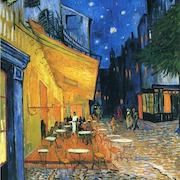
\includegraphics[width=20mm]{figures/cafe_terrace_at_night.png}}{original}
        \\
        \end{tabular}
\caption{ Best Images for $<num\_inds>$ = 10}
\normalsize
\end{figure}

\begin{figure}[H]
    \centering
    \begin{tabular}{c c}
        \subf{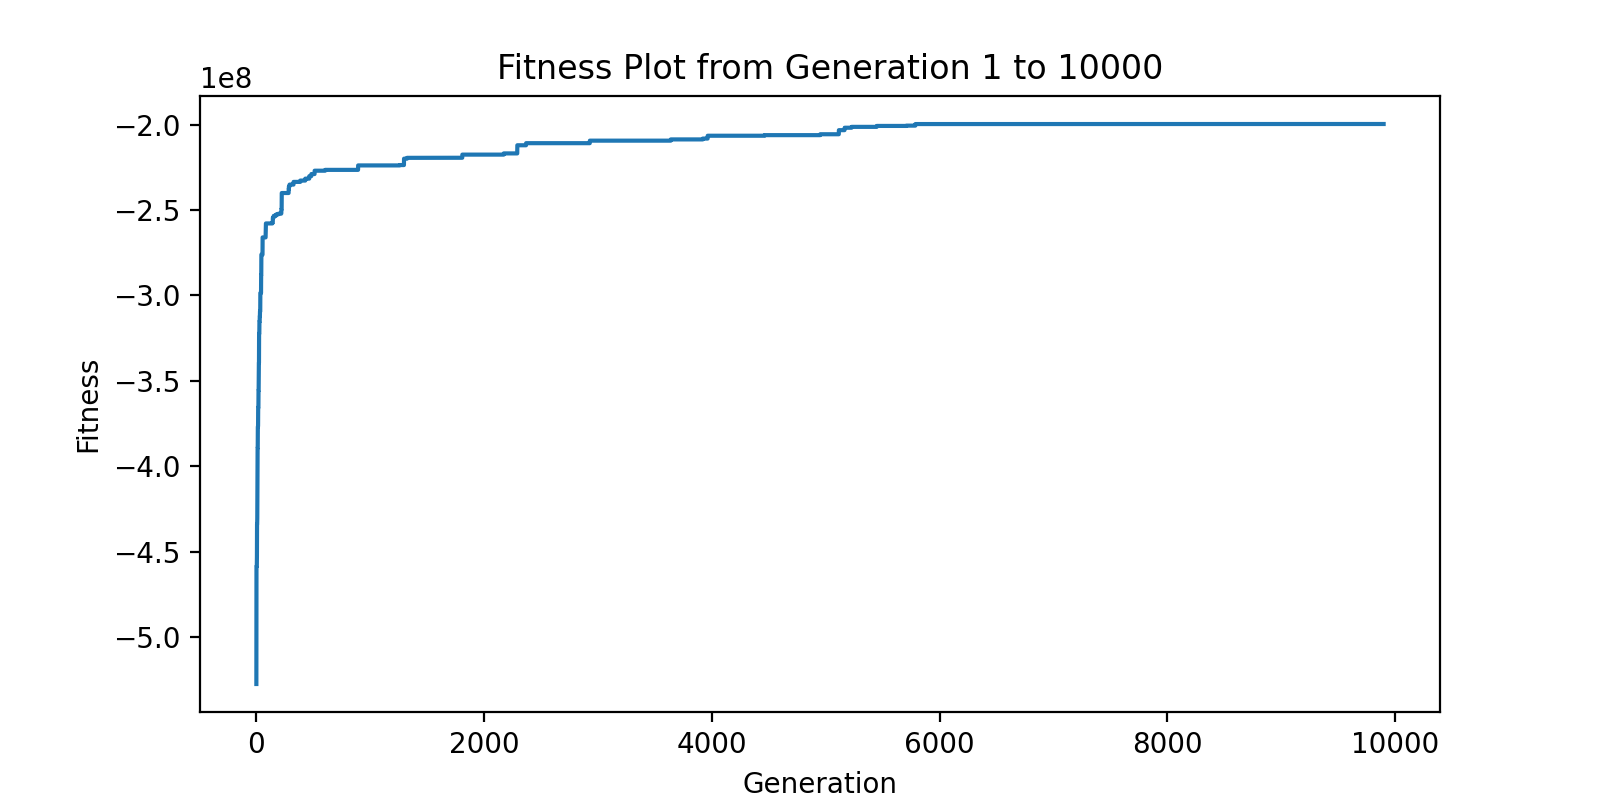
\includegraphics[width=75mm]{figures/ind-10/cafe_terrace_at_night_fitness.png}}{gens 1 to 10000}
        &
        \subf{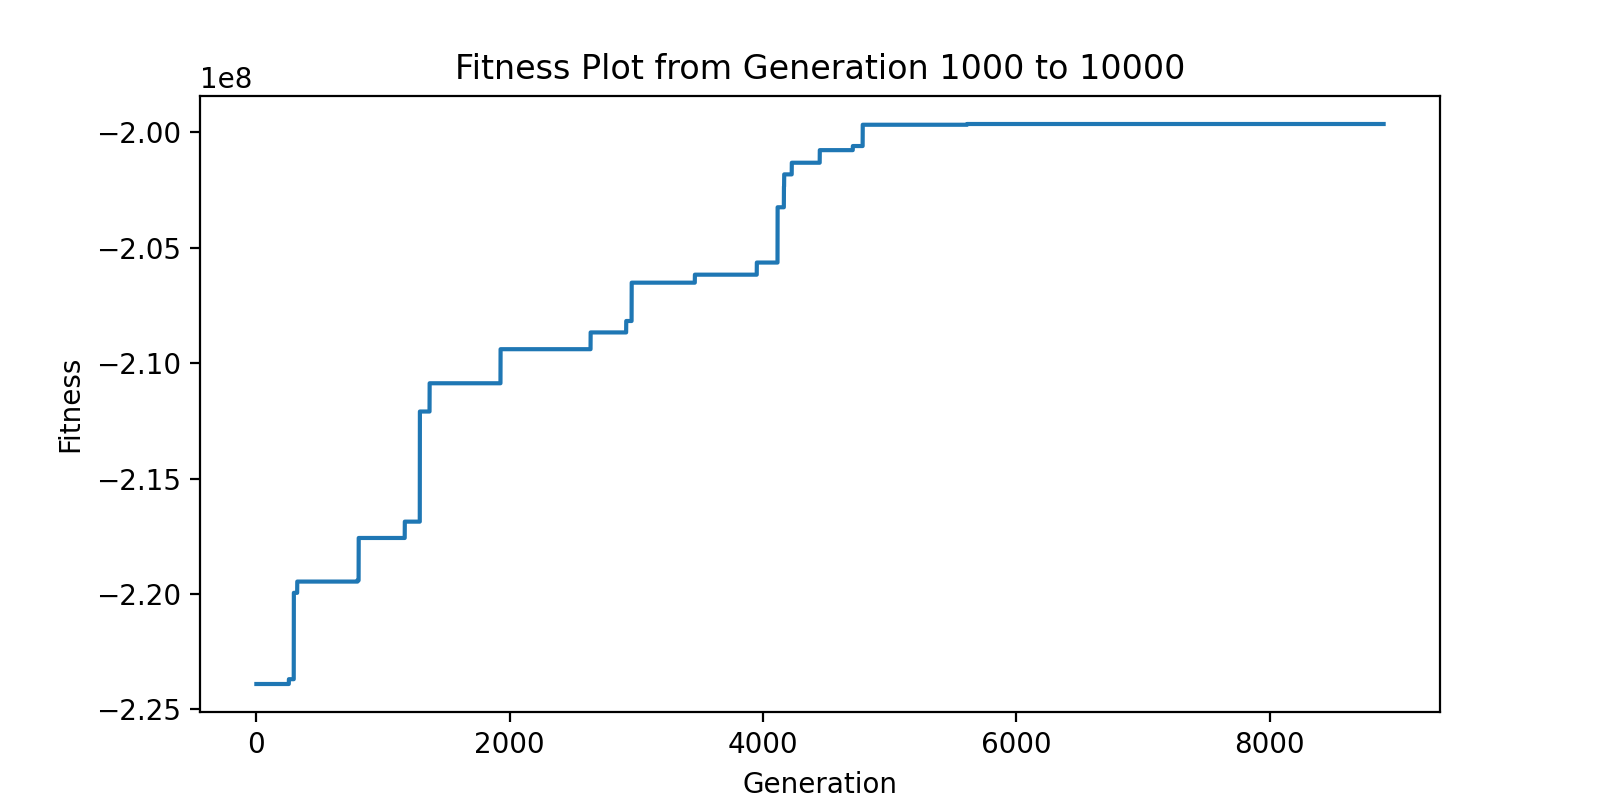
\includegraphics[width=75mm]{figures/ind-10/cafe_terrace_at_night_fitness_1000.png}}{gens 1000 to 10000}
        \\
        \end{tabular}
\caption{ Fitness Plots for $<num\_inds>$ = 10}
\normalsize
\end{figure}

\subsubsection{\textbf{Number of Individuals  = 40}}

\begin{figure}[H]
    \centering
    \begin{tabular}{c c c c c c}
          \subf{
\includegraphics[width=20mm]{figures/ind-40/cafe_terrace_at_night_gen_0.png}}{gens 0}
        &
        \subf{
\includegraphics[width=20mm]{figures/ind-40/cafe_terrace_at_night_gen_999.png}}{gens 1000}
        &
        \subf{
\includegraphics[width=20mm]{figures/ind-40/cafe_terrace_at_night_gen_1999.png}}{gens 2000}
        &
        \subf{
\includegraphics[width=20mm]{figures/ind-40/cafe_terrace_at_night_gen_2999.png}}{gens 3000}
        &
        \subf{
\includegraphics[width=20mm]{figures/ind-40/cafe_terrace_at_night_gen_3999.png}}{gens 4000}
        &
        \subf{
\includegraphics[width=20mm]{figures/ind-40/cafe_terrace_at_night_gen_4999.png}}{gens 5000}
        \\
        \end{tabular}
    \begin{tabular}{c c c c c c}
        \subf{
\includegraphics[width=20mm]{figures/ind-40/cafe_terrace_at_night_gen_5999.png}}{gens 6000}
        &
        \subf{
\includegraphics[width=20mm]{figures/ind-40/cafe_terrace_at_night_gen_6999.png}}{gens 7000}
        &
        \subf{\includegraphics[width=20mm]{figures/ind-40/cafe_terrace_at_night_gen_7999.png}}{gens 8000}
        &
        \subf{\includegraphics[width=20mm]{figures/ind-40/cafe_terrace_at_night_gen_8999.png}}{gens 9000}
        &
        \subf{\includegraphics[width=20mm]{figures/ind-40/cafe_terrace_at_night_gen_9999.png}}{gens 10000}
        &
        \subf{\includegraphics[width=20mm]{figures/cafe_terrace_at_night.png}}{original}
        \\
        \end{tabular}
\caption{ Best Images for $<num\_inds>$ = 40}
\normalsize
\end{figure}

\begin{figure}[H]
    \centering
    \begin{tabular}{c c}
        \subf{\includegraphics[width=75mm]{figures/ind-40/cafe_terrace_at_night_fitness.png}}{gens 1 to 10000}
        &
        \subf{\includegraphics[width=75mm]{figures/ind-40/cafe_terrace_at_night_fitness_1000.png}}{gens 1000 to 10000}
        \\
        \end{tabular}
\caption{ Fitness Plots for $<num\_inds>$ = 40}
\normalsize
\end{figure}

\subsubsection{\textbf{Number of Individuals  = 60}}

\begin{figure}[H]
    \centering
    \begin{tabular}{c c c c c c}
          \subf{\includegraphics[width=20mm]{figures/ind-60/cafe_terrace_at_night_gen_0.png}}{gens 0}
        &
        \subf{\includegraphics[width=20mm]{figures/ind-60/cafe_terrace_at_night_gen_999.png}}{gens 1000}
        &
        \subf{\includegraphics[width=20mm]{figures/ind-60/cafe_terrace_at_night_gen_1999.png}}{gens 2000}
        &
        \subf{\includegraphics[width=20mm]{figures/ind-60/cafe_terrace_at_night_gen_2999.png}}{gens 3000}
        &
        \subf{\includegraphics[width=20mm]{figures/ind-60/cafe_terrace_at_night_gen_3999.png}}{gens 4000}
        &
        \subf{\includegraphics[width=20mm]{figures/ind-60/cafe_terrace_at_night_gen_4999.png}}{gens 5000}
        \\
        \end{tabular}
    \begin{tabular}{c c c c c c}
        \subf{\includegraphics[width=20mm]{figures/ind-60/cafe_terrace_at_night_gen_5999.png}}{gens 6000}
        &
        \subf{\includegraphics[width=20mm]{figures/ind-60/cafe_terrace_at_night_gen_6999.png}}{gens 7000}
        &
        \subf{\includegraphics[width=20mm]{figures/ind-60/cafe_terrace_at_night_gen_7999.png}}{gens 8000}
        &
        \subf{\includegraphics[width=20mm]{figures/ind-60/cafe_terrace_at_night_gen_8999.png}}{gens 9000}
        &
        \subf{\includegraphics[width=20mm]{figures/ind-60/cafe_terrace_at_night_gen_9999.png}}{gens 10000}
        &
        \subf{\includegraphics[width=20mm]{figures/cafe_terrace_at_night.png}}{original}
        \\
        \end{tabular}
\caption{ Best Images for $<num\_inds>$ = 60}
\normalsize
\end{figure}

\begin{figure}[H]
    \centering
    \begin{tabular}{c c}
        \subf{\includegraphics[width=75mm]{figures/ind-60/cafe_terrace_at_night_fitness.png}}{gens 1 to 10000}
        &
        \subf{\includegraphics[width=75mm]{figures/ind-60/cafe_terrace_at_night_fitness_1000.png}}{gens 1000 to 10000}
        \\
        \end{tabular}
\caption{ Fitness Plots for $<num\_inds>$ = 60}
\normalsize
\end{figure}

A larger population size has better chance in exploring the solution space and finding the global optimum.
However, it also means that the algorithm will take more time to converge.
The smaller population size has better advantage in exploitation, that is searching around the promising regions of the solution space.

\medskip


A larger population size helps a faster convergence, that means that the algorithm is able to find the optimal solution in less number of generations, eventhougn the algorithm takes more processing power.
\medskip

Solution quality is also affected by the population size, we can see from the examples that the fitness plots of the larger population size is more smooth and predictable.

\subsection{\textbf{\Large Number of Genes \(<num\_genes>\)}}

The number of individuals is the size of the population. The individuals are used to generate next generation.
Higher the number of individuals, the more diverse the starting population is.

\subsubsection{\textbf{Number of Genes  = 15}}
\begin{figure}[H]
    \centering
    \begin{tabular}{c c c c c c}
          \subf{\includegraphics[width=20mm]{figures/genes-15/cafe_terrace_at_night_gen_0.png}}{gens 0}
        &
        \subf{\includegraphics[width=20mm]{figures/genes-15/cafe_terrace_at_night_gen_999.png}}{gens 1000}
        &
        \subf{\includegraphics[width=20mm]{figures/genes-15/cafe_terrace_at_night_gen_1999.png}}{gens 2000}
        &
        \subf{\includegraphics[width=20mm]{figures/genes-15/cafe_terrace_at_night_gen_2999.png}}{gens 3000}
        &
        \subf{\includegraphics[width=20mm]{figures/genes-15/cafe_terrace_at_night_gen_3999.png}}{gens 4000}
        &
        \subf{\includegraphics[width=20mm]{figures/genes-15/cafe_terrace_at_night_gen_4999.png}}{gens 5000}
        \\
        \end{tabular}
    \begin{tabular}{c c c c c c}
        \subf{\includegraphics[width=20mm]{figures/genes-15/cafe_terrace_at_night_gen_5999.png}}{gens 6000}
        &
        \subf{\includegraphics[width=20mm]{figures/genes-15/cafe_terrace_at_night_gen_6999.png}}{gens 7000}
        &
        \subf{\includegraphics[width=20mm]{figures/genes-15/cafe_terrace_at_night_gen_7999.png}}{gens 8000}
        &
        \subf{\includegraphics[width=20mm]{figures/genes-15/cafe_terrace_at_night_gen_8999.png}}{gens 9000}
        &
        \subf{\includegraphics[width=20mm]{figures/genes-15/cafe_terrace_at_night_gen_9999.png}}{gens 10000}
        &
        \subf{\includegraphics[width=20mm]{figures/cafe_terrace_at_night.png}}{original}
        \\
        \end{tabular}
\caption{ Best Images for $<num\_genes>$ = 15}
\normalsize
\end{figure}

\begin{figure}[H]
    \centering
    \begin{tabular}{c c}
        \subf{\includegraphics[width=75mm]{figures/genes-15/cafe_terrace_at_night_fitness.png}}{gens 1 to 10000}
        &
        \subf{\includegraphics[width=75mm]{figures/genes-15/cafe_terrace_at_night_fitness_1000.png}}{gens 1000 to 10000}
        \\
        \end{tabular}
\caption{ Fitness Plots for $<num\_genes>$ = 15}
\normalsize
\end{figure}

\subsubsection{\textbf{Number of Genes  = 30}}
\begin{figure}[H]
    \centering
    \begin{tabular}{c c c c c c}
          \subf{\includegraphics[width=20mm]{figures/genes-30/cafe_terrace_at_night_gen_0.png}}{gens 0}
        &
        \subf{\includegraphics[width=20mm]{figures/genes-30/cafe_terrace_at_night_gen_999.png}}{gens 1000}
        &
        \subf{\includegraphics[width=20mm]{figures/genes-30/cafe_terrace_at_night_gen_1999.png}}{gens 2000}
        &
        \subf{\includegraphics[width=20mm]{figures/genes-30/cafe_terrace_at_night_gen_2999.png}}{gens 3000}
        &
        \subf{\includegraphics[width=20mm]{figures/genes-30/cafe_terrace_at_night_gen_3999.png}}{gens 4000}
        &
        \subf{\includegraphics[width=20mm]{figures/genes-30/cafe_terrace_at_night_gen_4999.png}}{gens 5000}
        \\
        \end{tabular}
    \begin{tabular}{c c c c c c}
        \subf{\includegraphics[width=20mm]{figures/genes-30/cafe_terrace_at_night_gen_5999.png}}{gens 6000}
        &
        \subf{\includegraphics[width=20mm]{figures/genes-30/cafe_terrace_at_night_gen_6999.png}}{gens 7000}
        &
        \subf{\includegraphics[width=20mm]{figures/genes-30/cafe_terrace_at_night_gen_7999.png}}{gens 8000}
        &
        \subf{\includegraphics[width=20mm]{figures/genes-30/cafe_terrace_at_night_gen_8999.png}}{gens 9000}
        &
        \subf{\includegraphics[width=20mm]{figures/genes-30/cafe_terrace_at_night_gen_9999.png}}{gens 10000}
        &
        \subf{\includegraphics[width=20mm]{figures/cafe_terrace_at_night.png}}{original}
        \\
        \end{tabular}
\caption{ Best Images for $<num\_genes>$ = 30}
\normalsize
\end{figure}

\begin{figure}[H]
    \centering
    \begin{tabular}{c c}
        \subf{\includegraphics[width=75mm]{figures/genes-30/cafe_terrace_at_night_fitness.png}}{gens 1 to 10000}
        &
        \subf{\includegraphics[width=75mm]{figures/genes-30/cafe_terrace_at_night_fitness_1000.png}}{gens 1000 to 10000}
        \\
        \end{tabular}
\caption{ Fitness Plots for $<num\_genes>$ = 30}
\normalsize
\end{figure}

\subsubsection{\textbf{Number of Genes  = 80}}
\begin{figure}[H]
    \centering
    \begin{tabular}{c c c c c c}
          \subf{\includegraphics[width=20mm]{figures/genes-80/cafe_terrace_at_night_gen_0.png}}{gens 0}
        &
        \subf{\includegraphics[width=20mm]{figures/genes-80/cafe_terrace_at_night_gen_999.png}}{gens 1000}
        &
        \subf{\includegraphics[width=20mm]{figures/genes-80/cafe_terrace_at_night_gen_1999.png}}{gens 2000}
        &
        \subf{\includegraphics[width=20mm]{figures/genes-80/cafe_terrace_at_night_gen_2999.png}}{gens 3000}
        &
        \subf{\includegraphics[width=20mm]{figures/genes-80/cafe_terrace_at_night_gen_3999.png}}{gens 4000}
        &
        \subf{\includegraphics[width=20mm]{figures/genes-80/cafe_terrace_at_night_gen_4999.png}}{gens 5000}
        \\
        \end{tabular}
    \begin{tabular}{c c c c c c}
        \subf{\includegraphics[width=20mm]{figures/genes-80/cafe_terrace_at_night_gen_5999.png}}{gens 6000}
        &
        \subf{\includegraphics[width=20mm]{figures/genes-80/cafe_terrace_at_night_gen_6999.png}}{gens 7000}
        &
        \subf{\includegraphics[width=20mm]{figures/genes-80/cafe_terrace_at_night_gen_7999.png}}{gens 8000}
        &
        \subf{\includegraphics[width=20mm]{figures/genes-80/cafe_terrace_at_night_gen_8999.png}}{gens 9000}
        &
        \subf{\includegraphics[width=20mm]{figures/genes-80/cafe_terrace_at_night_gen_9999.png}}{gens 10000}
        &
        \subf{\includegraphics[width=20mm]{figures/cafe_terrace_at_night.png}}{original}
        \\
        \end{tabular}
\caption{ Best Images for $<num\_genes>$ = 80}
\normalsize
\end{figure}

\begin{figure}[H]
    \centering
    \begin{tabular}{c c}
        \subf{\includegraphics[width=75mm]{figures/genes-80/cafe_terrace_at_night_fitness.png}}{gens 1 to 10000}
        &
        \subf{\includegraphics[width=75mm]{figures/genes-80/cafe_terrace_at_night_fitness_1000.png}}{gens 1000 to 10000}
        \\
        \end{tabular}
\caption{ Fitness Plots for $<num\_genes>$ = 80}
\normalsize
\end{figure}

\subsubsection{\textbf{Number of Genes  = 120}}
\begin{figure}[H]
    \centering
    \begin{tabular}{c c c c c c}
          \subf{\includegraphics[width=20mm]{figures/genes-120/cafe_terrace_at_night_gen_0.png}}{gens 0}
        &
        \subf{\includegraphics[width=20mm]{figures/genes-120/cafe_terrace_at_night_gen_999.png}}{gens 1000}
        &
        \subf{\includegraphics[width=20mm]{figures/genes-120/cafe_terrace_at_night_gen_1999.png}}{gens 2000}
        &
        \subf{\includegraphics[width=20mm]{figures/genes-120/cafe_terrace_at_night_gen_2999.png}}{gens 3000}
        &
        \subf{\includegraphics[width=20mm]{figures/genes-120/cafe_terrace_at_night_gen_3999.png}}{gens 4000}
        &
        \subf{\includegraphics[width=20mm]{figures/genes-120/cafe_terrace_at_night_gen_4999.png}}{gens 5000}
        \\
        \end{tabular}
    \begin{tabular}{c c c c c c}
        \subf{\includegraphics[width=20mm]{figures/genes-120/cafe_terrace_at_night_gen_5999.png}}{gens 6000}
        &
        \subf{\includegraphics[width=20mm]{figures/genes-120/cafe_terrace_at_night_gen_6999.png}}{gens 7000}
        &
        \subf{\includegraphics[width=20mm]{figures/genes-120/cafe_terrace_at_night_gen_7999.png}}{gens 8000}
        &
        \subf{\includegraphics[width=20mm]{figures/genes-120/cafe_terrace_at_night_gen_8999.png}}{gens 9000}
        &
        \subf{\includegraphics[width=20mm]{figures/genes-120/cafe_terrace_at_night_gen_9999.png}}{gens 10000}
        &
        \subf{\includegraphics[width=20mm]{figures/cafe_terrace_at_night.png}}{original}
        \\
        \end{tabular}
\caption{ Best Images for $<num\_genes>$ = 120}
\normalsize
\end{figure}

\begin{figure}[H]
    \centering
    \begin{tabular}{c c}
        \subf{\includegraphics[width=75mm]{figures/genes-120/cafe_terrace_at_night_fitness.png}}{gens 1 to 10000}
        &
        \subf{\includegraphics[width=75mm]{figures/genes-120/cafe_terrace_at_night_fitness_1000.png}}{gens 1000 to 10000}
        \\
        \end{tabular}
\caption{ Fitness Plots for $<num\_genes>$ = 120}
\normalsize
\end{figure}









\subsection{\Large \textbf{Tournament Size \(<tm\_size>\)}}
\normalsize

The number of individuals is the size of the population. The individuals are used to generate next generation.
Higher the number of individuals, the more diverse the starting population is.

\subsubsection{\textbf{Tournament Size = 2}}
\begin{figure}[H]
    \centering
    \begin{tabular}{c c c c c c}
          \subf{\includegraphics[width=20mm]{figures/tm-2/cafe_terrace_at_night_gen_0.png}}{gens 0}
        &
        \subf{\includegraphics[width=20mm]{figures/tm-2/cafe_terrace_at_night_gen_999.png}}{gens 1000}
        &
        \subf{\includegraphics[width=20mm]{figures/tm-2/cafe_terrace_at_night_gen_1999.png}}{gens 2000}
        &
        \subf{\includegraphics[width=20mm]{figures/tm-2/cafe_terrace_at_night_gen_2999.png}}{gens 3000}
        &
        \subf{\includegraphics[width=20mm]{figures/tm-2/cafe_terrace_at_night_gen_3999.png}}{gens 4000}
        &
        \subf{\includegraphics[width=20mm]{figures/tm-2/cafe_terrace_at_night_gen_4999.png}}{gens 5000}
        \\
        \end{tabular}
    \begin{tabular}{c c c c c c}
        \subf{\includegraphics[width=20mm]{figures/tm-2/cafe_terrace_at_night_gen_5999.png}}{gens 6000}
        &
        \subf{\includegraphics[width=20mm]{figures/tm-2/cafe_terrace_at_night_gen_6999.png}}{gens 7000}
        &
        \subf{\includegraphics[width=20mm]{figures/tm-2/cafe_terrace_at_night_gen_7999.png}}{gens 8000}
        &
        \subf{\includegraphics[width=20mm]{figures/tm-2/cafe_terrace_at_night_gen_8999.png}}{gens 9000}
        &
        \subf{\includegraphics[width=20mm]{figures/tm-2/cafe_terrace_at_night_gen_9999.png}}{gens 10000}
        &
        \subf{\includegraphics[width=20mm]{figures/cafe_terrace_at_night.png}}{original}
        \\
        \end{tabular}
\caption{ Best Images for $<tm\_size>$ = 2}
\normalsize
\end{figure}

\begin{figure}[H]
    \centering
    \begin{tabular}{c c}
        \subf{\includegraphics[width=75mm]{figures/tm-2/cafe_terrace_at_night_fitness.png}}{gens 1 to 10000}
        &
        \subf{\includegraphics[width=75mm]{figures/tm-2/cafe_terrace_at_night_fitness_1000.png}}{gens 1000 to 10000}
        \\
        \end{tabular}
\caption{ Fitness Plots for $<tm\_size>$ = 2}
\normalsize
\end{figure}

\subsubsection{\textbf{Tournament Size = 8}}
\begin{figure}[H]
    \centering
    \begin{tabular}{c c c c c c}
          \subf{\includegraphics[width=20mm]{figures/tm-8/cafe_terrace_at_night_gen_0.png}}{gens 0}
        &
        \subf{\includegraphics[width=20mm]{figures/tm-8/cafe_terrace_at_night_gen_999.png}}{gens 1000}
        &
        \subf{\includegraphics[width=20mm]{figures/tm-8/cafe_terrace_at_night_gen_1999.png}}{gens 2000}
        &
        \subf{\includegraphics[width=20mm]{figures/tm-8/cafe_terrace_at_night_gen_2999.png}}{gens 3000}
        &
        \subf{\includegraphics[width=20mm]{figures/tm-8/cafe_terrace_at_night_gen_3999.png}}{gens 4000}
        &
        \subf{\includegraphics[width=20mm]{figures/tm-8/cafe_terrace_at_night_gen_4999.png}}{gens 5000}
        \\
        \end{tabular}
    \begin{tabular}{c c c c c c}
        \subf{\includegraphics[width=20mm]{figures/tm-8/cafe_terrace_at_night_gen_5999.png}}{gens 6000}
        &
        \subf{\includegraphics[width=20mm]{figures/tm-8/cafe_terrace_at_night_gen_6999.png}}{gens 7000}
        &
        \subf{\includegraphics[width=20mm]{figures/tm-8/cafe_terrace_at_night_gen_7999.png}}{gens 8000}
        &
        \subf{\includegraphics[width=20mm]{figures/tm-8/cafe_terrace_at_night_gen_8999.png}}{gens 9000}
        &
        \subf{\includegraphics[width=20mm]{figures/tm-8/cafe_terrace_at_night_gen_9999.png}}{gens 10000}
        &
        \subf{\includegraphics[width=20mm]{figures/cafe_terrace_at_night.png}}{original}
        \\
        \end{tabular}
\caption{ Best Images for $<tm\_size>$ = 8}
\normalsize
\end{figure}

\begin{figure}[H]
    \centering
    \begin{tabular}{c c}
        \subf{\includegraphics[width=75mm]{figures/tm-8/cafe_terrace_at_night_fitness.png}}{gens 1 to 10000}
        &
        \subf{\includegraphics[width=75mm]{figures/tm-8/cafe_terrace_at_night_fitness_1000.png}}{gens 1000 to 10000}
        \\
        \end{tabular}
\caption{ Fitness Plots for $<tm\_size>$ = 8}
\normalsize
\end{figure}

\subsubsection{\textbf{Tournament Size = 16}}
\begin{figure}[H]
    \centering
    \begin{tabular}{c c c c c c}
          \subf{\includegraphics[width=20mm]{figures/tm-16/cafe_terrace_at_night_gen_0.png}}{gens 0}
        &
        \subf{\includegraphics[width=20mm]{figures/tm-16/cafe_terrace_at_night_gen_999.png}}{gens 1000}
        &
        \subf{\includegraphics[width=20mm]{figures/tm-16/cafe_terrace_at_night_gen_1999.png}}{gens 2000}
        &
        \subf{\includegraphics[width=20mm]{figures/tm-16/cafe_terrace_at_night_gen_2999.png}}{gens 3000}
        &
        \subf{\includegraphics[width=20mm]{figures/tm-16/cafe_terrace_at_night_gen_3999.png}}{gens 4000}
        &
        \subf{\includegraphics[width=20mm]{figures/tm-16/cafe_terrace_at_night_gen_4999.png}}{gens 5000}
        \\
        \end{tabular}
    \begin{tabular}{c c c c c c}
        \subf{\includegraphics[width=20mm]{figures/tm-16/cafe_terrace_at_night_gen_5999.png}}{gens 6000}
        &
        \subf{\includegraphics[width=20mm]{figures/tm-16/cafe_terrace_at_night_gen_6999.png}}{gens 7000}
        &
        \subf{\includegraphics[width=20mm]{figures/tm-16/cafe_terrace_at_night_gen_7999.png}}{gens 8000}
        &
        \subf{\includegraphics[width=20mm]{figures/tm-16/cafe_terrace_at_night_gen_8999.png}}{gens 9000}
        &
        \subf{\includegraphics[width=20mm]{figures/tm-16/cafe_terrace_at_night_gen_9999.png}}{gens 10000}
        &
        \subf{\includegraphics[width=20mm]{figures/cafe_terrace_at_night.png}}{original}
        \\
        \end{tabular}
\caption{ Best Images for $<tm\_size>$ = 16}
\normalsize
\end{figure}

\begin{figure}[H]
    \centering
    \begin{tabular}{c c}
        \subf{\includegraphics[width=75mm]{figures/tm-16/cafe_terrace_at_night_fitness.png}}{gens 1 to 10000}
        &
        \subf{\includegraphics[width=75mm]{figures/tm-16/cafe_terrace_at_night_fitness_1000.png}}{gens 1000 to 10000}
        \\
        \end{tabular}
\caption{ Fitness Plots for $<tm\_size>$ = 16}
\normalsize
\end{figure}










\subsection{\Large \textbf{Fraction of Elites \(<frac\_elites>\)}}
\normalsize

The number of individuals is the size of the population. The individuals are used to generate next generation.
Higher the number of individuals, the more diverse the starting population is.

\subsubsection{\textbf{Fraction of Elites = 0.04}}
\begin{figure}[H]
    \centering
    \begin{tabular}{c c c c c c}
          \subf{\includegraphics[width=20mm]{figures/elites-0.04/cafe_terrace_at_night_gen_0.png}}{gens 0}
        &
        \subf{\includegraphics[width=20mm]{figures/elites-0.04/cafe_terrace_at_night_gen_999.png}}{gens 1000}
        &
        \subf{\includegraphics[width=20mm]{figures/elites-0.04/cafe_terrace_at_night_gen_1999.png}}{gens 2000}
        &
        \subf{\includegraphics[width=20mm]{figures/elites-0.04/cafe_terrace_at_night_gen_2999.png}}{gens 3000}
        &
        \subf{\includegraphics[width=20mm]{figures/elites-0.04/cafe_terrace_at_night_gen_3999.png}}{gens 4000}
        &
        \subf{\includegraphics[width=20mm]{figures/elites-0.04/cafe_terrace_at_night_gen_4999.png}}{gens 5000}
        \\
        \end{tabular}
    \begin{tabular}{c c c c c c}
        \subf{\includegraphics[width=20mm]{figures/elites-0.04/cafe_terrace_at_night_gen_5999.png}}{gens 6000}
        &
        \subf{\includegraphics[width=20mm]{figures/elites-0.04/cafe_terrace_at_night_gen_6999.png}}{gens 7000}
        &
        \subf{\includegraphics[width=20mm]{figures/elites-0.04/cafe_terrace_at_night_gen_7999.png}}{gens 8000}
        &
        \subf{\includegraphics[width=20mm]{figures/elites-0.04/cafe_terrace_at_night_gen_8999.png}}{gens 9000}
        &
        \subf{\includegraphics[width=20mm]{figures/elites-0.04/cafe_terrace_at_night_gen_9999.png}}{gens 10000}
        &
        \subf{\includegraphics[width=20mm]{figures/cafe_terrace_at_night.png}}{original}
        \\
        \end{tabular}
\caption{ Best Images for $<frac\_elites>$ = 0.04}
\normalsize
\end{figure}

\begin{figure}[H]
    \centering
    \begin{tabular}{c c}
        \subf{\includegraphics[width=75mm]{figures/elites-0.04/cafe_terrace_at_night_fitness.png}}{gens 1 to 10000}
        &
        \subf{\includegraphics[width=75mm]{figures/elites-0.04/cafe_terrace_at_night_fitness_1000.png}}{gens 1000 to 10000}
        \\
        \end{tabular}
\caption{ Fitness Plots for $<frac\_elites>$ = 0.04}
\normalsize
\end{figure}


\subsubsection{\textbf{Fraction of Elites = 0.35}}
\begin{figure}[H]
    \centering
    \begin{tabular}{c c c c c c}
          \subf{\includegraphics[width=20mm]{figures/elites-0.35/cafe_terrace_at_night_gen_0.png}}{gens 0}
        &
        \subf{\includegraphics[width=20mm]{figures/elites-0.35/cafe_terrace_at_night_gen_999.png}}{gens 1000}
        &
        \subf{\includegraphics[width=20mm]{figures/elites-0.35/cafe_terrace_at_night_gen_1999.png}}{gens 2000}
        &
        \subf{\includegraphics[width=20mm]{figures/elites-0.35/cafe_terrace_at_night_gen_2999.png}}{gens 3000}
        &
        \subf{\includegraphics[width=20mm]{figures/elites-0.35/cafe_terrace_at_night_gen_3999.png}}{gens 4000}
        &
        \subf{\includegraphics[width=20mm]{figures/elites-0.35/cafe_terrace_at_night_gen_4999.png}}{gens 5000}
        \\
        \end{tabular}
    \begin{tabular}{c c c c c c}
        \subf{\includegraphics[width=20mm]{figures/elites-0.35/cafe_terrace_at_night_gen_5999.png}}{gens 6000}
        &
        \subf{\includegraphics[width=20mm]{figures/elites-0.35/cafe_terrace_at_night_gen_6999.png}}{gens 7000}
        &
        \subf{\includegraphics[width=20mm]{figures/elites-0.35/cafe_terrace_at_night_gen_7999.png}}{gens 8000}
        &
        \subf{\includegraphics[width=20mm]{figures/elites-0.35/cafe_terrace_at_night_gen_8999.png}}{gens 9000}
        &
        \subf{\includegraphics[width=20mm]{figures/elites-0.35/cafe_terrace_at_night_gen_9999.png}}{gens 10000}
        &
        \subf{\includegraphics[width=20mm]{figures/cafe_terrace_at_night.png}}{original}
        \\
        \end{tabular}
\caption{ Best Images for $<frac\_elites>$ = 0.35}
\normalsize
\end{figure}

\begin{figure}[H]
    \centering
    \begin{tabular}{c c}
        \subf{\includegraphics[width=75mm]{figures/elites-0.35/cafe_terrace_at_night_fitness.png}}{gens 1 to 10000}
        &
        \subf{\includegraphics[width=75mm]{figures/elites-0.35/cafe_terrace_at_night_fitness_1000.png}}{gens 1000 to 10000}
        \\
        \end{tabular}
\caption{ Fitness Plots for $<frac\_elites>$ = 0.35}
\normalsize
\end{figure}










\subsection{\Large \textbf{Fraction of Parents \(<frac\_parents>\)}}
\normalsize

The number of individuals is the size of the population. The individuals are used to generate next generation.
Higher the number of individuals, the more diverse the starting population is.

\subsubsection{\textbf{Fraction of Parents = 0.15}}
\begin{figure}[H]
    \centering
    \begin{tabular}{c c c c c c}
          \subf{\includegraphics[width=20mm]{figures/parents-0.15/cafe_terrace_at_night_gen_0.png}}{gens 0}
        &
        \subf{\includegraphics[width=20mm]{figures/parents-0.15/cafe_terrace_at_night_gen_999.png}}{gens 1000}
        &
        \subf{\includegraphics[width=20mm]{figures/parents-0.15/cafe_terrace_at_night_gen_1999.png}}{gens 2000}
        &
        \subf{\includegraphics[width=20mm]{figures/parents-0.15/cafe_terrace_at_night_gen_2999.png}}{gens 3000}
        &
        \subf{\includegraphics[width=20mm]{figures/parents-0.15/cafe_terrace_at_night_gen_3999.png}}{gens 4000}
        &
        \subf{\includegraphics[width=20mm]{figures/parents-0.15/cafe_terrace_at_night_gen_4999.png}}{gens 5000}
        \\
        \end{tabular}
    \begin{tabular}{c c c c c c}
        \subf{\includegraphics[width=20mm]{figures/parents-0.15/cafe_terrace_at_night_gen_5999.png}}{gens 6000}
        &
        \subf{\includegraphics[width=20mm]{figures/parents-0.15/cafe_terrace_at_night_gen_6999.png}}{gens 7000}
        &
        \subf{\includegraphics[width=20mm]{figures/parents-0.15/cafe_terrace_at_night_gen_7999.png}}{gens 8000}
        &
        \subf{\includegraphics[width=20mm]{figures/parents-0.15/cafe_terrace_at_night_gen_8999.png}}{gens 9000}
        &
        \subf{\includegraphics[width=20mm]{figures/parents-0.15/cafe_terrace_at_night_gen_9999.png}}{gens 10000}
        &
        \subf{\includegraphics[width=20mm]{figures/cafe_terrace_at_night.png}}{original}
        \\
        \end{tabular}
\caption{ Best Images for $<frac\_parents>$ = 0.15}
\normalsize
\end{figure}

\begin{figure}[H]
    \centering
    \begin{tabular}{c c}
        \subf{\includegraphics[width=75mm]{figures/parents-0.15/cafe_terrace_at_night_fitness.png}}{gens 1 to 10000}
        &
        \subf{\includegraphics[width=75mm]{figures/parents-0.15/cafe_terrace_at_night_fitness_1000.png}}{gens 1000 to 10000}
        \\
        \end{tabular}
\caption{ Fitness Plots for $<frac\_parents>$ = 0.15}
\normalsize
\end{figure}


\subsubsection{\textbf{Fraction of Parents = 0.3}}
\begin{figure}[H]
    \centering
    \begin{tabular}{c c c c c c}
          \subf{\includegraphics[width=20mm]{figures/parents-0.3/cafe_terrace_at_night_gen_0.png}}{gens 0}
        &
        \subf{\includegraphics[width=20mm]{figures/parents-0.3/cafe_terrace_at_night_gen_999.png}}{gens 1000}
        &
        \subf{\includegraphics[width=20mm]{figures/parents-0.3/cafe_terrace_at_night_gen_1999.png}}{gens 2000}
        &
        \subf{\includegraphics[width=20mm]{figures/parents-0.3/cafe_terrace_at_night_gen_2999.png}}{gens 3000}
        &
        \subf{\includegraphics[width=20mm]{figures/parents-0.3/cafe_terrace_at_night_gen_3999.png}}{gens 4000}
        &
        \subf{\includegraphics[width=20mm]{figures/parents-0.3/cafe_terrace_at_night_gen_4999.png}}{gens 5000}
        \\
        \end{tabular}
    \begin{tabular}{c c c c c c}
        \subf{\includegraphics[width=20mm]{figures/parents-0.3/cafe_terrace_at_night_gen_5999.png}}{gens 6000}
        &
        \subf{\includegraphics[width=20mm]{figures/parents-0.3/cafe_terrace_at_night_gen_6999.png}}{gens 7000}
        &
        \subf{\includegraphics[width=20mm]{figures/parents-0.3/cafe_terrace_at_night_gen_7999.png}}{gens 8000}
        &
        \subf{\includegraphics[width=20mm]{figures/parents-0.3/cafe_terrace_at_night_gen_8999.png}}{gens 9000}
        &
        \subf{\includegraphics[width=20mm]{figures/parents-0.3/cafe_terrace_at_night_gen_9999.png}}{gens 10000}
        &
        \subf{\includegraphics[width=20mm]{figures/cafe_terrace_at_night.png}}{original}
        \\
        \end{tabular}
\caption{ Best Images for $<frac\_parents>$ = 0.3}
\normalsize
\end{figure}

\begin{figure}[H]
    \centering
    \begin{tabular}{c c}
        \subf{\includegraphics[width=75mm]{figures/parents-0.3/cafe_terrace_at_night_fitness.png}}{gens 1 to 10000}
        &
        \subf{\includegraphics[width=75mm]{figures/parents-0.3/cafe_terrace_at_night_fitness_1000.png}}{gens 1000 to 10000}
        \\
        \end{tabular}
\caption{ Fitness Plots for $<frac\_parents>$ = 0.3}
\normalsize
\end{figure}


\subsubsection{\textbf{Fraction of Parents = 0.75}}
\begin{figure}[H]
    \centering
    \begin{tabular}{c c c c c c}
          \subf{\includegraphics[width=20mm]{figures/parents-0.75/cafe_terrace_at_night_gen_0.png}}{gens 0}
        &
        \subf{\includegraphics[width=20mm]{figures/parents-0.75/cafe_terrace_at_night_gen_999.png}}{gens 1000}
        &
        \subf{\includegraphics[width=20mm]{figures/parents-0.75/cafe_terrace_at_night_gen_1999.png}}{gens 2000}
        &
        \subf{\includegraphics[width=20mm]{figures/parents-0.75/cafe_terrace_at_night_gen_2999.png}}{gens 3000}
        &
        \subf{\includegraphics[width=20mm]{figures/parents-0.75/cafe_terrace_at_night_gen_3999.png}}{gens 4000}
        &
        \subf{\includegraphics[width=20mm]{figures/parents-0.75/cafe_terrace_at_night_gen_4999.png}}{gens 5000}
        \\
        \end{tabular}
    \begin{tabular}{c c c c c c}
        \subf{\includegraphics[width=20mm]{figures/parents-0.75/cafe_terrace_at_night_gen_5999.png}}{gens 6000}
        &
        \subf{\includegraphics[width=20mm]{figures/parents-0.75/cafe_terrace_at_night_gen_6999.png}}{gens 7000}
        &
        \subf{\includegraphics[width=20mm]{figures/parents-0.75/cafe_terrace_at_night_gen_7999.png}}{gens 8000}
        &
        \subf{\includegraphics[width=20mm]{figures/parents-0.75/cafe_terrace_at_night_gen_8999.png}}{gens 9000}
        &
        \subf{\includegraphics[width=20mm]{figures/parents-0.75/cafe_terrace_at_night_gen_9999.png}}{gens 10000}
        &
        \subf{\includegraphics[width=20mm]{figures/cafe_terrace_at_night.png}}{original}
        \\
        \end{tabular}
\caption{ Best Images for $<frac\_parents>$ = 0.75}
\normalsize
\end{figure}

\begin{figure}[H]
    \centering
    \begin{tabular}{c c}
        \subf{\includegraphics[width=75mm]{figures/parents-0.75/cafe_terrace_at_night_fitness.png}}{gens 1 to 10000}
        &
        \subf{\includegraphics[width=75mm]{figures/parents-0.75/cafe_terrace_at_night_fitness_1000.png}}{gens 1000 to 10000}
        \\
        \end{tabular}
\caption{ Fitness Plots for $<frac\_parents>$ = 0.75}
\normalsize
\end{figure}










\subsection{\Large \textbf{Mutation Probability \(<mutation\_prob>\)}}
\normalsize

The number of individuals is the size of the population. The individuals are used to generate next generation.
Higher the number of individuals, the more diverse the starting population is.

\subsubsection{\textbf{Mutation Probability = 0.1}}
\begin{figure}[H]
    \centering
    \begin{tabular}{c c c c c c}
          \subf{\includegraphics[width=20mm]{figures/prob-0.1/cafe_terrace_at_night_gen_0.png}}{gens 0}
        &
        \subf{\includegraphics[width=20mm]{figures/prob-0.1/cafe_terrace_at_night_gen_999.png}}{gens 1000}
        &
        \subf{\includegraphics[width=20mm]{figures/prob-0.1/cafe_terrace_at_night_gen_1999.png}}{gens 2000}
        &
        \subf{\includegraphics[width=20mm]{figures/prob-0.1/cafe_terrace_at_night_gen_2999.png}}{gens 3000}
        &
        \subf{\includegraphics[width=20mm]{figures/prob-0.1/cafe_terrace_at_night_gen_3999.png}}{gens 4000}
        &
        \subf{\includegraphics[width=20mm]{figures/prob-0.1/cafe_terrace_at_night_gen_4999.png}}{gens 5000}
        \\
        \end{tabular}
    \begin{tabular}{c c c c c c}
        \subf{\includegraphics[width=20mm]{figures/prob-0.1/cafe_terrace_at_night_gen_5999.png}}{gens 6000}
        &
        \subf{\includegraphics[width=20mm]{figures/prob-0.1/cafe_terrace_at_night_gen_6999.png}}{gens 7000}
        &
        \subf{\includegraphics[width=20mm]{figures/prob-0.1/cafe_terrace_at_night_gen_7999.png}}{gens 8000}
        &
        \subf{\includegraphics[width=20mm]{figures/prob-0.1/cafe_terrace_at_night_gen_8999.png}}{gens 9000}
        &
        \subf{\includegraphics[width=20mm]{figures/prob-0.1/cafe_terrace_at_night_gen_9999.png}}{gens 10000}
        &
        \subf{\includegraphics[width=20mm]{figures/cafe_terrace_at_night.png}}{original}
        \\
        \end{tabular}
\caption{ Best Images for $<mutation\_prob>$ = 0.1}
\normalsize
\end{figure}

\begin{figure}[H]
    \centering
    \begin{tabular}{c c}
        \subf{\includegraphics[width=75mm]{figures/prob-0.1/cafe_terrace_at_night_fitness.png}}{gens 1 to 10000}
        &
        \subf{\includegraphics[width=75mm]{figures/prob-0.1/cafe_terrace_at_night_fitness_1000.png}}{gens 1000 to 10000}
        \\
        \end{tabular}
\caption{ Fitness Plots for $<mutation\_prob>$ = 0.1}
\normalsize
\end{figure}

\subsubsection{\textbf{Mutation Probability = 0.4}}
\begin{figure}[H]
    \centering
    \begin{tabular}{c c c c c c}
          \subf{\includegraphics[width=20mm]{figures/prob-0.4/cafe_terrace_at_night_gen_0.png}}{gens 0}
        &
        \subf{\includegraphics[width=20mm]{figures/prob-0.4/cafe_terrace_at_night_gen_999.png}}{gens 1000}
        &
        \subf{\includegraphics[width=20mm]{figures/prob-0.4/cafe_terrace_at_night_gen_1999.png}}{gens 2000}
        &
        \subf{\includegraphics[width=20mm]{figures/prob-0.4/cafe_terrace_at_night_gen_2999.png}}{gens 3000}
        &
        \subf{\includegraphics[width=20mm]{figures/prob-0.4/cafe_terrace_at_night_gen_3999.png}}{gens 4000}
        &
        \subf{\includegraphics[width=20mm]{figures/prob-0.4/cafe_terrace_at_night_gen_4999.png}}{gens 5000}
        \\
        \end{tabular}
    \begin{tabular}{c c c c c c}
        \subf{\includegraphics[width=20mm]{figures/prob-0.4/cafe_terrace_at_night_gen_5999.png}}{gens 6000}
        &
        \subf{\includegraphics[width=20mm]{figures/prob-0.4/cafe_terrace_at_night_gen_6999.png}}{gens 7000}
        &
        \subf{\includegraphics[width=20mm]{figures/prob-0.4/cafe_terrace_at_night_gen_7999.png}}{gens 8000}
        &
        \subf{\includegraphics[width=20mm]{figures/prob-0.4/cafe_terrace_at_night_gen_8999.png}}{gens 9000}
        &
        \subf{\includegraphics[width=20mm]{figures/prob-0.4/cafe_terrace_at_night_gen_9999.png}}{gens 10000}
        &
        \subf{\includegraphics[width=20mm]{figures/cafe_terrace_at_night.png}}{original}
        \\
        \end{tabular}
\caption{ Best Images for $<mutation\_prob>$ = 0.4}
\normalsize
\end{figure}

\begin{figure}[H]
    \centering
    \begin{tabular}{c c}
        \subf{\includegraphics[width=75mm]{figures/prob-0.4/cafe_terrace_at_night_fitness.png}}{gens 1 to 10000}
        &
        \subf{\includegraphics[width=75mm]{figures/prob-0.4/cafe_terrace_at_night_fitness_1000.png}}{gens 1000 to 10000}
        \\
        \end{tabular}
\caption{ Fitness Plots for $<mutation\_prob>$ = 0.4}
\normalsize
\end{figure}

\subsubsection{\textbf{Mutation Probability = 0.75}}
\begin{figure}[H]
    \centering
    \begin{tabular}{c c c c c c}
          \subf{\includegraphics[width=20mm]{figures/prob-0.75/cafe_terrace_at_night_gen_0.png}}{gens 0}
        &
        \subf{\includegraphics[width=20mm]{figures/prob-0.75/cafe_terrace_at_night_gen_999.png}}{gens 1000}
        &
        \subf{\includegraphics[width=20mm]{figures/prob-0.75/cafe_terrace_at_night_gen_1999.png}}{gens 2000}
        &
        \subf{\includegraphics[width=20mm]{figures/prob-0.75/cafe_terrace_at_night_gen_2999.png}}{gens 3000}
        &
        \subf{\includegraphics[width=20mm]{figures/prob-0.75/cafe_terrace_at_night_gen_3999.png}}{gens 4000}
        &
        \subf{\includegraphics[width=20mm]{figures/prob-0.75/cafe_terrace_at_night_gen_4999.png}}{gens 5000}
        \\
        \end{tabular}
    \begin{tabular}{c c c c c c}
        \subf{\includegraphics[width=20mm]{figures/prob-0.75/cafe_terrace_at_night_gen_5999.png}}{gens 6000}
        &
        \subf{\includegraphics[width=20mm]{figures/prob-0.75/cafe_terrace_at_night_gen_6999.png}}{gens 7000}
        &
        \subf{\includegraphics[width=20mm]{figures/prob-0.75/cafe_terrace_at_night_gen_7999.png}}{gens 8000}
        &
        \subf{\includegraphics[width=20mm]{figures/prob-0.75/cafe_terrace_at_night_gen_8999.png}}{gens 9000}
        &
        \subf{\includegraphics[width=20mm]{figures/prob-0.75/cafe_terrace_at_night_gen_9999.png}}{gens 10000}
        &
        \subf{\includegraphics[width=20mm]{figures/cafe_terrace_at_night.png}}{original}
        \\
        \end{tabular}
\caption{ Best Images for $<mutation\_prob>$ = 0.75}
\normalsize
\end{figure}

\begin{figure}[H]
    \centering
    \begin{tabular}{c c}
        \subf{\includegraphics[width=75mm]{figures/prob-0.75/cafe_terrace_at_night_fitness.png}}{gens 1 to 10000}
        &
        \subf{\includegraphics[width=75mm]{figures/prob-0.75/cafe_terrace_at_night_fitness_1000.png}}{gens 1000 to 10000}
        \\
        \end{tabular}
\caption{ Fitness Plots for $<mutation\_prob>$ = 0.75}
\normalsize
\end{figure}






\subsection{\Large \textbf{Mutation Type \(<mutation\_type>\)}}
\normalsize

The number of individuals is the size of the population. The individuals are used to generate next generation.
Higher the number of individuals, the more diverse the starting population is.

\subsubsection{\textbf{Mutation Type = unguided}}
\begin{figure}[H]
    \centering
    \begin{tabular}{c c c c c c}
          \subf{\includegraphics[width=20mm]{figures/type-1/cafe_terrace_at_night_gen_0.png}}{gens 0}
        &
        \subf{\includegraphics[width=20mm]{figures/type-1/cafe_terrace_at_night_gen_999.png}}{gens 1000}
        &
        \subf{\includegraphics[width=20mm]{figures/type-1/cafe_terrace_at_night_gen_1999.png}}{gens 2000}
        &
        \subf{\includegraphics[width=20mm]{figures/type-1/cafe_terrace_at_night_gen_2999.png}}{gens 3000}
        &
        \subf{\includegraphics[width=20mm]{figures/type-1/cafe_terrace_at_night_gen_3999.png}}{gens 4000}
        &
        \subf{\includegraphics[width=20mm]{figures/type-1/cafe_terrace_at_night_gen_4999.png}}{gens 5000}
        \\
        \end{tabular}
    \begin{tabular}{c c c c c c}
        \subf{\includegraphics[width=20mm]{figures/type-1/cafe_terrace_at_night_gen_5999.png}}{gens 6000}
        &
        \subf{\includegraphics[width=20mm]{figures/type-1/cafe_terrace_at_night_gen_6999.png}}{gens 7000}
        &
        \subf{\includegraphics[width=20mm]{figures/type-1/cafe_terrace_at_night_gen_7999.png}}{gens 8000}
        &
        \subf{\includegraphics[width=20mm]{figures/type-1/cafe_terrace_at_night_gen_8999.png}}{gens 9000}
        &
        \subf{\includegraphics[width=20mm]{figures/type-1/cafe_terrace_at_night_gen_9999.png}}{gens 10000}
        &
        \subf{\includegraphics[width=20mm]{figures/cafe_terrace_at_night.png}}{original}
        \\
        \end{tabular}
\caption{ Best Images for $<mutation\_type>$ = unguided}
\normalsize
\end{figure}

\begin{figure}[H]
    \centering
    \begin{tabular}{c c}
        \subf{\includegraphics[width=75mm]{figures/type-1/cafe_terrace_at_night_fitness.png}}{gens 1 to 10000}
        &
        \subf{\includegraphics[width=75mm]{figures/type-1/cafe_terrace_at_night_fitness_1000.png}}{gens 1000 to 10000}
        \\
        \end{tabular}
\caption{ Fitness Plots for $<mutation\_type>$ = unguided}
\normalsize
\end{figure}


















% \begin{figure}[H]
%     \centering
%     \includegraphics[width=0.9\textwidth, trim={0 0cm 0 0cm}]{figures/num_inds.png}
%     \caption{Effect of the number of individuals on the output quality}
%     \label{fig:inds}




% An ANNs classifier trained with cross-entropy loss approximates a conditional probability distribution. Specifically, given an input vector, the classifier outputs a probability distribution over the possible classes that the input could belong to. The cross-entropy loss is defined as the negative log-likelihood of the correct class given the input.
% The reason why cross-entropy loss is used to approximate this function is that it is well-suited for optimizing models that output probability distributions. The loss encourages the model to assign a high probability to the correct class and low probabilities to the incorrect classes, which is exactly what we want from a classifier. The negative log-likelihood also has desirable properties such as being continuous and differentiable, making it easier to optimize using gradient-based methods.

% Bulleted lists may be included and should look like this:
% \begin{itemize}[]
% \item First point
% \item Second point
% \item And so on
% \end{itemize}

\vspace{-0.5em}
\subsection{\textbf{Gradient Computation}}
High number of iterations, when the difference between the weights are small, the gradient calculation can be made with basic slope calculation.
\vspace{-0.7em}
\begin{equation*}
    \begin{array}{l}
         \textrm{$ \textstyle  \gamma \nabla \mathcal{L}_{\omega_{k}} = \omega_{k} - \omega_{k+1}  $} \\
        \hspace{10em} hence, \\
         \displaystyle \textrm{$  \nabla_{\omega} \mathcal{L}\big\rvert_{\omega = \omega_{k}} = \frac{\omega_{k} - \omega_{k+1}}{\gamma}$}   \\
    \end{array}
\end{equation*}

\subsection{\textbf{Some Training Parameters and Basic Parameter Calculations}}
\begin{enumerate}
    \item The batch refers to a subset of the training data that is used to compute the weights for one iteration. More specifically, the batch size is the number of training samples in a batch.
 The epoch on the other hand refers to the number of times the entire training data is used to update the weights. In training, there are generally multiple epoch iterations where the weights are updated with different batches/subsets of the training data.
    \item For the $N$ number of training samples, the number of batches per epoch is $N/B$, where $B$ is the batch size. A little side note that the solution is rounded up to the higher integer if $N/B$ is not an integer.
    \item For the optimization iterations, such as SGD, for $E$ number of epochs, the total number of iterations is $E \times N/B$. Again, a practical side note states that the $N/B$ is rounded up to the higher integer.
\end{enumerate}
\subsection{\textbf{Computing Number of Parameters of ANN Classifiers}}
\begin{enumerate}
    \item Starting from the initial layer of the MLP, we have $D_{in}$ number of input neurons and $H_1$ number of neurons in first hidden layer. Also there are biases associated with 
each neuron. Therefore, the number of parameters of the each layer is,
    \vspace{-0.5cm}
    \begin{equation*}
    \begin{array}{r}
    \textrm{Input Layer} = D_{in} \times H_{1} \ +\ H_{1} \\
    \textrm{Hidden Layers}= H_1 \times H_2 + H_2\\
    \cdot \cdot \cdot \hspace{2em} \\
    \textrm{More Hidden Layers} = H_{k-1} \times H_k + H_k\\
    \textrm{Output Layer} = H_{k} \times D_{out} \ +\ D_{out} \\
    \end{array}
    \end{equation*}

    \vspace{-0.25cm}
    The total sum can be written as, where $K$ is the number of hidden layers.
    \vspace{-0.5cm}
    \begin{equation*}
        \textrm{Total Number of Parameters} = D_{in}\times H_1 + \sum_{k=2}^{K} (H_{k-1} \times H_k + H_k) + H_k \times D_{out} +  D_{out}
    \end{equation*}
    \vspace{-0.25cm}

    \item CNN structure is more complicated. The number of parameters of a CNN layer is calculated as follows:
    
    For the input layer, the number of parameters is,
    \vspace{-0.5cm}
    \begin{equation*}
        \textrm{Input Layer} = [(H_{in}-H_1+1) \times (W_{in}-W_1+1)\times C_{in} \times C_1 ]+ C_1
    \end{equation*}

    \vspace{-0.25cm}
    where $H_{in}$ and $W_{in}$ are the height and width of the input image, and $C_{in}$ is the number of channels of the input image.
    Each input of layer is the output of the previous layer.
    There exist also biases associated with each neuron added.
    For the convolutional layers, the number of parameters is calculated as,
    \vspace{-0.5cm}
    \begin{equation*}
        \begin{array}{c}
            \displaystyle \textrm{Convolutional Layer} = [(H_k-H_{k+1}+1) \times (W_k-W_{k+1}+1) \times C_{k} \times C_{k+1}] + C_{k+1} \\
            \\
            \displaystyle \textrm{Combination of all layers is,} \\
            \displaystyle \textrm{Convolutional Layers} = \sum_{k=1}^{K} [(H_k-H_{k+1}+1) \times (W_k-W_{k+1}+1) \times C_{k} \times C_{k+1}] + C_{k+1} \\ 
        \end{array}
    \end{equation*}

    \vspace{-0.25cm}
    Here all the parameters are summed up. The output is assumed to be the last index of the array.
    The final equation for the total number of parameters is,
    \vspace{-0.5cm}

    
    \begin{equation*}
        \hspace{-1cm} \textrm{Total Parameters} = [(H_k-H_{k+1}+1) \times (W_k-W_{k+1}+1) \times C_{k} \times C_{k+1}] + C_{k+1} + \sum_{k=1}^{K} [(H_k-H_{k+1}+1) \times (W_k-W_{k+1}+1) \times C_{k} \times C_{k+1}] + C_{k+1}
    \end{equation*}

    \vspace{-0.25cm}

\end{enumerate}

% All tables should be numbered with Arabic numerals. Every table should have a caption. Headings should be placed above tables, left justified. Only horizontal lines should be used within a table, to distinguish the column headings from the body of the table, and immediately above and below the table. Tables must be embedded into the text and not supplied separately. Below is an example which the authors may find useful.

% \begin{table}[h]
% \caption{ An example of a table.}
% \begin{tabular*}{\hsize}{@{\extracolsep{\fill}}lll@{}}
% \toprule
% An example of a column heading & Column A ({\it{t}}) & Column B ({\it{t}})\\
% \colrule
% And an entry &   1 &  2\\
% And another entry  & 3 &  4\\
% And another entry &  5 &  6\\
% \botrule
% \end{tabular*}
% \end{table}

% %\enlargethispage{12pt}

\section{\textbf{Implementing a Convolutional Layer with NumPy}}

The section involves implementing conv2d function using NumPy for forward propagation and testing it on a small batch of MNIST dataset.
We downloaded and loaded input and kernel files, and created an output image using the part2Plots function.
The implementation code can be found in the appendix named my\_conv2d.py.
We confirmed the correctness of our implementation by the output image.
% References must be listed at the end of the paper. Do not begin them on a new page unless this is absolutely necessary. Authors should ensure that every reference in the text appears in the list of references and vice versa. Indicate references by \cite{Massimo2011} or \cite{Massimo2012} or \cite{Thomas2015} in the text.
% Some examples of how your references should be listed are given at the end of this template in the `References' section, which will allow you to assemble your reference list according to the correct format and font size.

% Reference generation by using bibliography style commands for LaTeX template only.

% The author may use ``elsarticle-harv.bst'' as per the style required in document. The sample bib file could be referred. 
% If the author may using bibstyle for providing references author must comment the bibliography section in TeX file, Bibtex will generate the reference automatically.

% If the author may not able to view the references in output same could be done by copying the bibliography section from ``filename.bbl'' file and paste in TeX file.



\subsection{\textbf{Experimental Work}}
The generated output for the convolution over the MNIST dataset is shown in Figure \ref{fig:output}.



% \begin{figure}[H]
%     \centering
%     \includegraphics[width=0.5\textwidth, trim={0 5cm 0 5cm}]{figures/output.png}
%     \caption{Convolution over the number 8 of the MNIST dataset}
%     \label{fig:output}
% \end{figure}

\vspace{-0.5cm}
\subsection{\textbf{Results and Discussion}}
\begin{enumerate}
    \item The Convolutional Neural Networks are important for couple of reasons.
    First of all, when the input shape of the CNN is selected as 2D, it is well suited image processing.
    Second, the CNN is able to learn the spatial features of the input image. This also means that the CNN is able to learn and extract the features of the input image without any manual work.
    CNN's are also able to recognize the features of the input image even if the input image is rotated or scaled.
    Since the features are extracted from image, partial occlusion of the image affect the performance of the CNN less.
    \item The kernel of a Convolutional Layer  is essentially a matrix of weights that is convolved (inversely correlated) over with the input data to extract features.
    The size of the kernel refers to the number of rows and columns in the matrix. It corresponds to the reception of the filter, meaning that higher sizes can extract more complex features. 
    
    \item The output image shows that the convolution of pre-presented kernels for the number 8 of the MNIST dataset. Basically each filter is convoled over the images to grasp different meanings. Each column is another kernel with each row is different input image.
    
    \item The numbers in the same column look like each other since they both have a representation of the same number and the same kernel is able to extract the features related to the number 8 other than the specific image.
    
    \item The numbers in the same row look different althougn the input image the same. This is because the kernels are different and they are able to extract different features from the same image.
    
    \item For more specific examples, the third column kernel represents that an 8 has two "islands" of white patches in the middle but the size, shape and location of these pathes differ for each 8 altough all of them represent the same thing in a different manner.
     Another column such as 6, implies the white track like feature of the number 8. In this sense some features are more dinstinctive than other however when different of these combined make the action work even though they do not seem to represent a clear feature.
     This is similar to human behaviour as we associate the similar patterns to the general inputs and this is the importance of the convolutaional layers, the features can be learned in a sense.
\end{enumerate}

\section{\textbf{Experimenting ANN Architectures}}

\subsection{\textbf{Experimental Work}}

This experimental work focuses on testing various Artificial Neural Network (ANN) architectures for a classification task. The models will use adaptive moment estimation (Adam) with default parameters for the optimizer. The datasets will be preprocessed and split into three sets: training, validation, and testing. The ANN architectures to be tested are ‘mlp 1’, ‘mlp 2’, ‘cnn 3’, ‘cnn 4’, and ‘cnn 5’, each with their specific layers.
For each architecture, the ANN will be trained for 15 epochs, and training loss, accuracy, validation accuracy, and test accuracy will be recorded. The best test accuracy and weights of the first layer will be recorded, and a dictionary object will be created and saved for each architecture.
Performance comparison plots will be created, and the weights of the first layer of all architectures will be visualized.

% \begin{figure}[H]
%     \centering
%     \includegraphics[width=0.9\textwidth, trim={0 0cm 0 0cm}]{figures/aa.png}
%     \caption{Performance Comparison Plots for the ANN Architectures} 
%     \label{fig:perf}
% \end{figure}

\subsection{\textbf{Results and Discussion}}
\begin{enumerate}
    \item Generalization performance refers to the ability of the model to to classify the unseen data. It is used as the ability to recognize patterns and apply this knowledge to the new data.
    \item The plots showing the results with the "test" data show the generalization performance since the test data is not used in the training process and the model is not familiar with the test data.
    Validation data is also seemed to be a good indicator of the generalization performance. However, altough  the validation data is not directly used in training process, it is used to tune the parameters of the model. Therefore, the model is familiar with the validation data in a sense.
    The first two curves and the last x-y plot give hint about the comparative generalization performance since these show the results with the validation data.
    The third scatter plot on the other hand is used with the test data, hence have the correct generalization performance. However it only shows the best run hence the variety of the results are a topic of discussion and the plot does not show that information.

    \item Copmarative results show that the convolutional architectures perform better than the multi-layer perceptron architectures. This is because the convolutional layers are able to extract spatial features from the data with more grasping ability.
    The "mlp\_1" and "mlp\_2" are very similar in terms of performance although they have different size of parameters and number of layers.
    The "cnn\_3" and "cnn\_4" are also very similar again the latter has more layers. 
    The "cnn\_5" is more of a slow learner and could not get to the same level of performance as the "cnn\_4" but with more epochs it is seem to be able to surpass the "cnn\_4" since the gradient of the accuracy is increasing.

    \item Higher the number of parameters, it is generally easier for model to learn complex features. However it also means that the model is more prone to overfitting.
    This is because the model is able to learn the training data in more depth, like its noise characteristics not the required features. Hence, it is not able to generalize well.
    This is called overfitting, the models with higher parameters have more "memory" that they can memorize the unwanted characteristics that is specific to the training data.
    Another aspect is the distribution of the parameters, the convolutaional layers use the parameters more eficiently and make more of the increased number of parameters without easily falling into overfitting trap.
    
    \item The depth of the architecture is also relevelant with the distribution of the parameters, how they organized in an architecture. The models with more depth are able to learn more complex features as well, however they are harder to train in terms of computation.
    The extremum of depth parameter results in not overfitting but underfitting. This is because the model is not able to learn the features of the data in depth and generalize well.

    % \begin{figure}
    %     \centering
    %     \begin{tabular}{c c}
    %     \subf{\includegraphics[width=72mm]{figures/mlp_1_weights.png}}{a) mlp\_1}
    %     &
    %     \subf{\includegraphics[width=72mm]{figures/mlp_2_weights.png}}{b) mlp\_2}
    %     \\
    %     \end{tabular}
    %     \begin{tabular}{c c c}
    %     \subf{\includegraphics[width=45mm]{figures/cnn_3_weights.png}}{c) cnn\_3}
    %     &
    %     \subf{\includegraphics[width=45mm]{figures/cnn_4_weights.png}}{d) cnn\_4}
    %     &
    %     \subf{\includegraphics[width=45mm]{figures/cnn_5_weights.png}}{e) cnn\_5}
    %     \\
    %     \end{tabular}
    % \end{figure}
    % \label{fig:weights}

    \item The first layer weights of the MLP structure has high resolution, and can be interpreted as some curves and horizontal lines are perceived.
    for the CNN structures the weights are more abstract but these architectures have more depth hence a meaning can be found when these are all evaluated together.
    \item It is early to say that the units are related with the classes with initial layer weights but horizontal lines can be the plane wing identifier with the tail and body sections are interpreted in the latter layers.
    \item At this stage, with the more information on MLP's first layer, it is more interpretable.
    \item For each arhchiecture, the depth is increased as explained in previous sections. CNN have an advantage in classification of an image input over the MLP. The higher depth suggests that the CNN is able to learn more complex features and generalize better.
    \item I would go with the CNN architecture for image classification task. More specifically "cnn\_4" which performs around the same as others with faster training and less parameters as "cnn\_5".
    
\end{enumerate}

\section{\textbf{Experimenting Activation Functions}}

\subsection{\textbf{Experimental Work}}

This section compares the performance of artificial neural networks (ANNs) using the rectified linear unit (ReLU) and logistic sigmoid activation functions, trained with stochastic gradient descent (SGD) on a constant learning rate of 0.01, 0.0 momentum, and a batch size of 50 samples.
For each architecture in section 3.1, two torch.nn.Module objects are created with ReLU and logistic sigmoid activations respectively. The ANNs are trained for 15 epochs, recording the training loss and magnitude of the loss gradient at every 10 steps.
The results are saved as dictionary objects with filenames prefixed with 'part4'.
Finally, performance comparison plots are generated.

% \begin{figure}[H]
%     \centering
%     \includegraphics[width=0.9\textwidth, trim={0 1cm 0 1cm}]{figures/bb.png}
%     \caption{Performance Comparison Plots for the Different Activation Functions over the Different Architectures.} 
%     \label{fig:act_fun}
% \end{figure}

\subsection{\textbf{Results and Discussion}}
\begin{enumerate}
    \item As the depth increases, the normalized gradient of the loss decreases. Also for the further steps it does not change much,
    meaning that the learning gets slower.
    The most complex model "cnn\_5" has the lower gradient of the lost for starting epochs. At a point, also loss gradient reduces after a peak value. This also suggests that the training will get slower.
    The shallow models "mlp\_1" and "mlp\_2" have relatively high gradients of loss. However, from the minimum loss plot, it is seen that the loss is not decreasing much after a point. This is due model is not deep enough to learn more of the features.

    \item Increasing with the depth, gradients start to become harder to calculate. This is because the gradients are calculated by backpropagation and the gradients of the previous layers are needed to calculate the gradients of the current layer. Increasing the complexity at each iteration.
    \item Bonus: Since the gradients are calculated from the weights, the unnormalized input can cause gradients to become very small and the learning could take longer.
    Also for different scales of inputs, the model can give bias to one or more features, which can also reduce the performance of both the training process and the overall system.
\end{enumerate}
\section{\textbf{Experimenting Learning Rate}}

\subsection{\textbf{Experimental Work}}
This section explores the effect of varying learning rates in the stochastic gradient descent (SGD) optimization method with a ReLU activation function, 0.0 momentum, and batch size of 50 samples. Three torch.nn.Module objects are created with initial learning rates of 0.1, 0.01, and 0.001, respectively, and trained for 20 epochs. The training loss and validation accuracy are recorded every 10 steps to form loss and accuracy curves.
Scheduled learning rate is then explored by training a classifier with a 0.1 learning rate until the epoch step where the validation accuracy stops increasing. The learning rate is then reduced and training continues for another 30 epochs. Finally, the test accuracy of the trained model is compared to the same model trained with Adam in section 3.1.

% \begin{figure}[H]
%     \centering
%     \includegraphics[width=0.9\textwidth, trim={0 1cm 0 1cm}]{figures/cc.png}
%     \caption{Performance Comparison Plots for the Different Learning Rates of "cnn\_4".} 
%     \label{fig:LR}
% \end{figure}

\subsection{\textbf{Results and Discussion}}
\begin{enumerate}
    \item Higher learning rates lead to faster convergence, however the model can skip the global minimum. Lower learning rates can lead to a slower convergernce.
    \item High learning rate might not get to the minimum point but oscillate around it. Lower has better chance to get to the minimum point.
    \item The scheduled learning rate iteratively reduces the learning rate, promising a better convergence with a better step count.
    \item With the scheduled learning rate, there is a jump at the epoch 7, which is the point where the learning rate is reduced.
    The next jump is at epoch 17, however the performance does not increase much after that, suggesting a minimal point is reached.
    One thing to notice that the training accuracy is higher than the respected model in part 3.1.
    But the validation accuracy is around the same at 66\%.

\end{enumerate}

% \begin{figure}[H]
%     \centering
%     \includegraphics[width=0.95\textwidth, trim={0 1cm 0 1cm}]{figures/cnn_4_SC_validation_acc.png}
%     \caption{Validation Accuracy with Scheduled Learning Rate for the "cnn\_4".} 
%     \label{fig:SC}
% \end{figure}

% \begin{figure}[H]
%     \centering
%     \includegraphics[width=0.95\textwidth, trim={0 1cm 0 1cm}]{figures/cnn_4_SC_training_loss.png}
%     \caption{Training Loss with Scheduled Learning Rate for the "cnn\_4".} 
%     \label{fig:SC2}
% \end{figure}

% Please title your files in this order `procedia acronym\_conference acronym\_authorslastname'.  Submit both the source file and the PDF to the Guest Editor.

% Artwork filenames should comply with the syntax ``aabbbbbb.ccc'', where:
% \begin{itemize}
% \item a = artwork component type
% \item b = manuscript reference code
% \item c = standard file extension

% Component types:
% \item gr = figure
% \item pl = plate
% \item sc = scheme
% \item fx = fixed graphic
% \end{itemize}


% \subsection{Footnotes}
% Footnotes should be avoided if possible. Necessary footnotes should be denoted in the text by consecutive superscript letters\footnote{Footnote text.}. The footnotes should be typed single spaced, and in smaller type size (8 pt), at the foot of the page in which they are mentioned, and separated from the main text by a one line space extending at the foot of the column. The `Els-footnote' style is available in the ``TeX Template'' for the text of the footnote.

% Please do not change the margins of the template as this can result in the footnote falling outside printing range.


% \section{Illustrations}
% All figures should be numbered with Arabic numerals (1,2,3,$\,\ldots.$). Every figure should have a caption. All\break photographs, schemas, graphs and diagrams are to be referred to as figures. Line drawings should be good\break quality scans or true electronic output. Low-quality scans are not acceptable. Figures must be embedded into the text and not supplied separately. In MS word input the figures must be properly coded. Preferred format of figures are PNG, JPEG, GIF etc. Lettering and symbols should be clearly defined either in the caption or in a legend provided as part of the figure. Figures should be placed at the top or bottom of a page wherever possible, as close as possible to the first reference to them in the paper. Please ensure that all the figures are of 300 DPI resolutions as this will facilitate good output.

% The figure number and caption should be typed below the illustration in 8 pt and left justified [{\bfseries\itshape Note:} one-line captions of length less than column width (or full typesetting width or oblong) centered]. For more guidelines and\break information to help you submit high quality artwork please visit: http://www.elsevier.com/artworkinstructions\break Artwork has no text along the side of it in the main body of the text. However, if two images fit next to each other, these may be placed next to each other to save space. For example, see Fig.~1.
% \begin{figure}[t]\vspace*{4pt}
% %\centerline{\includegraphics{fx1}\hspace*{5mm}\includegraphics{fx1}}
% %\centerline{\includegraphics{gr1}}
% \caption{(a) first picture; (b) second picture.}
% \end{figure}


% \section{Equations}
% Equations and formulae should be typed in MathType, and numbered consecutively with Arabic numerals in parentheses on the right hand side of the page (if referred to explicitly in the text). They should also be separated from the surrounding text by one space
% \begin{equation}
% \begin{array}{lcl}
% \displaystyle X_r &=& \displaystyle\dot{Q}^{''}_{rad}\left/\left(\dot{Q}^{''}_{rad} + \dot{Q}^{''}_{conv}\right)\right.\\[6pt]
% \displaystyle \rho &=& \displaystyle\frac{\vec{E}}{J_c(T={\rm const.})\cdot\left(P\cdot\left(\displaystyle\frac{\vec{E}}{E_c}\right)^m+(1-P)\right)}
% \end{array}
% \end{equation}


% \section{Online license transfer}
% All authors are required to complete the Procedia exclusive license transfer agreement before the article can be published, which they can do online. This transfer agreement enables Elsevier to protect the copyrighted material for the authors, but does not relinquish the authors' proprietary rights. The copyright transfer covers the exclusive rights to reproduce and distribute the article, including reprints, photographic reproductions, microfilm or any other reproductions of similar nature and translations. Authors are responsible for obtaining from the copyright holder, the permission to reproduce any figures for which copyright exists.

% \section*{Acknowledgements}

% Acknowledgements and Reference heading should be left justified, bold, with the first letter capitalized but have no numbers. Text below continues as normal.

% %% The Appendices part is started with the command \appendix;
% %% appendix sections are then done as normal sections
% %% \appendix

% %% \section{}
% %% \label{}

% \appendix
% \section{Python Scripts}


% \subsection{Example of a sub-heading within an appendix}
% There is also the option to include a subheading within the Appendix if you wish.
%% References
%%
%% Following citation commands can be used in the body text:
%% Usage of \cite is as follows:
%%   \cite{key}         ==>>  [#]
%%   \cite[chap. 2]{key} ==>> [#, chap. 2]
%%

%The citation must be used in following style: \cite{article-minimal} \cite{article-full} \cite{article-crossref} \cite{whole-journal}.
%% References with BibTeX database:

%\bibliography{xampl}
%\bibliographystyle{elsarticle-harv}


%% Authors are advised to use a BibTeX database file for their reference list.
%% The provided style file elsarticle-num.bst formats references in the required Procedia style

%% For references without a BibTeX database:

%  \begin{thebibliography}{}

%% \bibitem must have the following form:
%%   \bibitem{key}...
%%

% \bibitem{Massimo2011}
% {F}ilippini, Massimo, and Lester C. Hunt. (2011) ``Energy demand and
% energy efficiency in the OECD countries: a stochastic demand frontier
% approach." {\it Energy Journal} {\bf 32} (2): 59--80.
% \bibitem{Massimo2012}
% Filippini, Massimo, and Lester C. Hunt. (2012) ``US residential
% energy demand and energy efficiency: A stochastic demand frontier
% approach." {\it Energy Economics} {\bf 34} (5): 1484--1491.
% \bibitem{Thomas2015} 
% Weyman-Jones, Thomas, J\'{u}lia Mendon\c{c}a Boucinha, and Catarina
% Feteira In\'{a}cio. (2015) ``Measuring electric energy efficiency in
% Portuguese households: a tool for energy policy." {\it Management of Environmental Quality: An International Journal} {\bf 26} (3): 407--422.
% \bibitem{} 
% Saunders, Harry (2009) ``Theoretical Foundations of the Rebound Effect'', in Joanne Evans and Lester Hunt (eds) {\it International Handbook on the Economics of Energy}, Cheltenham, Edward Elgar
% \bibitem{} 
% Sorrell, Steve (2009) ``The Rebound Effect: definition and estimation'', in Joanne Evans and Lester Hunt (eds) {\it International Handbook on the Economics of Energy}, Cheltenham, Edward Elgar 
%  \end{thebibliography}

\clearpage

%%%% This page is for instructions only, once the article is finalize please omit the below text before creating the final PDF
\normalMode

% \section*{Instructions to Authors for LaTeX template:}

% \section{ZIP mode for LaTeX template:}

% The zip package is created as per the guide lines present on the URL http://www.elsevier.com/author-schemas/ preparing-crc-journal-articles-with-latex for creating the LaTeX zip file of Procedia LaTeX template.  The zip generally contains the following files:
% \begin{Itemize}[]\leftskip-17.7pt\labelsep3.3pt
% \item ecrc.sty
% \item  elsarticle.cls
% \item elsdoc.pdf
% \item .bst file
% \item Manuscript templates for use with these bibliographic styles
% \item  Generic and journal specific logos, etc.
% \end{Itemize}

% The LaTeX package is the main LaTeX template. All LaTeX support files are required for LaTeX pdf generation from the LaTeX template package. 

% {\bf Reference style .bst file used for collaboration support:} In the LaTeX template packages of all Procedia titles a new ``.bst'' file is used which supports collaborations downloaded from the path http://www.elsevier.com/author-schemas/the-elsarticle-latex-document-class

% \section{Reference style used in Computer Science:}
% \let\footnotesize\normalsize
% \hspace*{-10pt}\begin{tabular*}{\hsize}{@{}ll@{}}
% {\bf Title}&{\bf Reference style} \\[6pt]
% PROCS  & 3 Vancouver Numbered
% \end{tabular*}

\end{document}

%%
%% End of file `procs-template.tex'.
